\documentclass[12pt,a4paper,titlepage]{report}

% Document Info
%
\newcommand\AcademicTitle{Dynamic Performance Framework}
\newcommand\CommericalTitle{Iris}
\newcommand\Author{Dean Gaffney}
\newcommand\StudentID{20067423}
\newcommand\Date{December 2017}
\newcommand\Report{Status Report (Semester 2)}
\newcommand\Reader{Supervisor: Dr.~Kieran Murphy}
\newcommand\SecondReader{Second Reader: David Drohan}

\usepackage{fyp_document}

\newcommand*{\mybox}[2]{\colorbox{#1!30}{\parbox{.98\linewidth}{#2}}}
\newcommand{\q}[1]{``#1''}

\crefname{paragraph}{paragraph}{paragraphs}
\Crefname{paragraph}{Paragraph}{Paragraphs}

\begin{document}

\pagenumbering{roman}

% title page as per Ian's spec
\thispagestyle{empty}
\begin{center}
\mbox{}\vfill
{\fontsize{18pt}{20pt}\selectfont \bfseries \AcademicTitle}
\vfill
{\fontsize{14pt}{20pt}\selectfont \bfseries\itshape \CommericalTitle}
\vfill
{\fontsize{12pt}{20pt}\selectfont \bfseries \Report}
\vfill
{\fontsize{14pt}{20pt}\selectfont \bfseries \Author}
\vfill
{\fontsize{14pt}{20pt}\selectfont \bfseries \StudentID\ Panel 3}
\vfill
{\fontsize{14pt}{20pt}\selectfont \bfseries \Reader}
\vfill
{\fontsize{14pt}{20pt}\selectfont \bfseries \SecondReader}
\vfill
{\fontsize{14pt}{20pt}\selectfont \bfseries BSc (Hons) in Entertainment Systems}
\vfill
\end{center}
\clearpage

\tableofcontents
\listoftables
\listoffigures

% start of main matter
\clearpage
\pagenumbering{arabic}
\setcounter{page}{1}

\chapter{Abstract}

The aim of this project is the design a full implementation of a system for application performance monitoring. The proposed system, has the working title,  Iris.

On completion, Iris will provide users with a dynamic performance framework which will allow users to fully customise and centralise their application performance monitoring. This will be achieved through a web interface where a user can specify a schema for a specific application they wish to monitor. Once a schema has been set up, a REST endpoint will be generated for the application. This endpoint will allow a user to send their monitoring data from their desired application to the framework in the form of JSON (matching the specified schema). Iris will also contain features which allow a user to monitor and analyse incoming data, using an intelligent, fully customisable graph and dashboard builder. Iris will then visualise any received data in real time using to the appropriate dashboards using websockets. Iris will come with some out of the box scripts/applications that users can use to monitor typical tasks such as JVM (Java Virtual Machine) performance, Linux OS System Performance.

\chapter{Introduction}

\section{Motivation for Iris}

The motivation for this project comes from database and system performance issues that Onaware\footnote{Onaware is an international company that specialises in IAM (Identity and Access Management) and has offices with 20 staff in Waterford. More information on Onaware can be found at \url{https://onaware.com}.} has experienced in recent projects. It is often the case that they must deal with large amounts of identity data being aggregated into a third party system called `IIQ'.

Onaware has faced major issues with aggregating data in the past, in some cases it was taking up to five days, and sometimes they would fail halfway through meaning aggregations would have to be restarted, due to the amount of software involved it is hard to pinpoint what software is causing the issue.

In one such instance of aggregating data issues several attempts were made to rectify the performance issue such as optimising sql queries, increasing ram, multi threading tasks and increasing disk space, none of which worked. Due to the performance issue the IIQ instance became unusable so debugging the issue was not possible from inside the application and log files became so big that text editors would crash when trying to open them. In this case the issue turned out to be a customer putting size constraints on the database storing the aggregated data. While monitoring would not prevent such a mistake it would have reduced the time needed to locate the issue.

In response to difficulties in identifying performance issues Onaware have tried to monitor specific application elements. The aim at the time was to try and combine SQL, JVM and Operating System scripts to track the performance of the tools, however this approach is not very scalable and it would need to be reconfigured for future projects.

Iris is an attempt to solve this problem. Iris will allow a user create a new application monitor with little effort using a web interface, give the user a REST endpoint specific to the application for their scripts to target their data, and allow a user to monitor the data in real time using graphs and dashboards. The aim is to make the framework as flexible as possible and not specific to the issue Onaware faced, meaning a user can monitor any data they want from any application they want all they must do is send their data to a REST endpoint.

Users of Iris will consist of Onaware developers who will be monitoring IAM project data and generic tools which may be released to clients at a later time.

\section{Features List}
\subsection{Types of data}
numerical, categorical and textural

\chapter{Implementation}
During semester 1 a number of implementation were designed and tested. As a result the implementation described in
semester 1 required not further changes in thus semester. Hence, this section is fundamentally unchanged from that in
semester 1 report
Distinguish between subparts that were implemented (and so their overview here is similar to that in semester 1 report) and
subparts that were implemented during this semester (and so the overview here is new).
In this chapter the implementation of Iris is summarised. The components completed in semester were described in the
Semester 1 report and that summary is reproduced here (with minor modification) for completeness. The subsections dealing
with components implemented in semester 2 is fundamentally new. Table REF lists the components adn when they were completed.
\begin{center}
\begin{tabular}{llll}
Component                         & When prototyped  & When completed \\\hline
code framework/services  & Semester 1 & Semester 1 \\
schemas &\\
dashboards &\\
aggregation builder  &\\
data sources & \\
\end{tabular}
\end{center}

\section{Core Framework/Services}
In the Semester 1 report the design of Iris is described. Due to the testing of the designs in the first semester the final design needed no further modifications this semester. Hence the description of Iris given here follows closely that given in report 1.

\subsection{Description}
Iris will act as a web interface for a user to create an application monitor and allow the user to query and create personalised dashboards of their data through the use of Elasticsearch. A user may setup an application schema definition within Iris that matches the data they wish to monitor, a schema will consist of field names and corresponding data types specific to the application. Using the schema Iris will know what data to expect from the user. Once a schema is in place, Iris will generate a unique endpoint associated with the schema, this unique endpoint will be given to the user as a means of sending data to Iris. Data sent to the schema endpoint will be in JSON format and will conform to the schema definition created by the user in Iris.
\begin{figure}[H]
\begin{tcolorbox}
A user creates an application monitor for an SQL database, they may create a schema like the following:
\begin{minted}{yaml}
Schema Name: "SQL Monitor"
Schema Fields:
    -field name: "writeSpeed"
     fieldType: "double"
    -field name: "tableName"
     fieldType: "String"
\end{minted}
Iris will then expect a json object to come back in the form:
\begin{minted}{json}
{
	"writeSpeed": 3000,
	"tableName":  "students"
}
\end{minted}
\end{tcolorbox}
\caption{Example schema created for Iris.}
\end{figure}

Iris will take the users data and create data mappings \parencite{Elastic.co.Mapping} inside Elasticsearch, as well as insert any incoming data into the correct Elasticsearch index~\parencite{Elastic.co.Basic}. With a schema in place a user can route their data through Iris; turning Iris into a centralised area for monitoring application performance data. With Iris being the centralised location to route and view your data a user can write a data transformation script for incoming data. The advantage of this is that it can help reduce the need for applications being redeployed to view new data or to transform data.

\begin{figure}[H]
\begin{tcolorbox}

The user releases their application, and it is downloaded by 500 people. This data is now being sent from 500 instances of this application. To make any change to this data the developer must add in their desired field and and redeploy the app, those 500 users would then need to download an update for the application in order for it to take effect. The original JSON object passing through Iris looks like the following:
\begin{minted}{json}
{
	"firstName": "Dean",
	"lastName":  "Gaffney"
}
\end{minted}

In this example let's say the developer prefers to have the data mapped to a field called \q{fullName} which is all lowercase, the developer wants to avoid having to redeploy the app for one single field, instead the developer goes to Iris and applies a script to the schema. By running the script on incoming data the developer has made their desired change in a central location with no redeploys. The data may look like this after the developer has applied the script to the data:
\begin{minted}{json}
{
	"firstName": "Dean",
	"lastName":  "Gaffney",
	"fullName":  "Dean Gaffney"
}
\end{minted}
\end{tcolorbox}
\caption{Iris transforming data.}
\end{figure}

To aid performance monitoring, Iris will allow users to create personalised dashboards where they can create charts from their data and place them in the dashboard. This allows each user to have their own set of visualised data relative to them. To help a user see their data and charts rapidly an Elasticsearch aggregation~\parencite{Elastic.co.Aggregations} playground will be put into place in order to allow a user create charts and get results back immediately, this will help a user to plan their dashboard charts before setting them up. The playground will also allow a user to chain several aggregations together which will allow them to create complex queries without having to have any prior knowledge of how Elasticsearch works.

 
\subsection{Schemas}
Schemas in Iris have not changed from semester 1 in terms of their design, they are still used as a representation of a data source in Iris which is created by the user. However there were some improvements made on both the front and backend of Iris to make the creation and interaction of agents with schemas easier for the user. These improvements will be discussed in the following sections.
\subsubsection{Frontend}
This section will discuss the improvements made to the frontend of Iris in regards to the Schema section.

\paragraph{Schema Fields}
Iris now displays the Schema Fields in a table fashion and presents the user with the name and data types of all the fields in the schema.
\begin{figure}[H]
\begin{tcolorbox}
\begin{center}
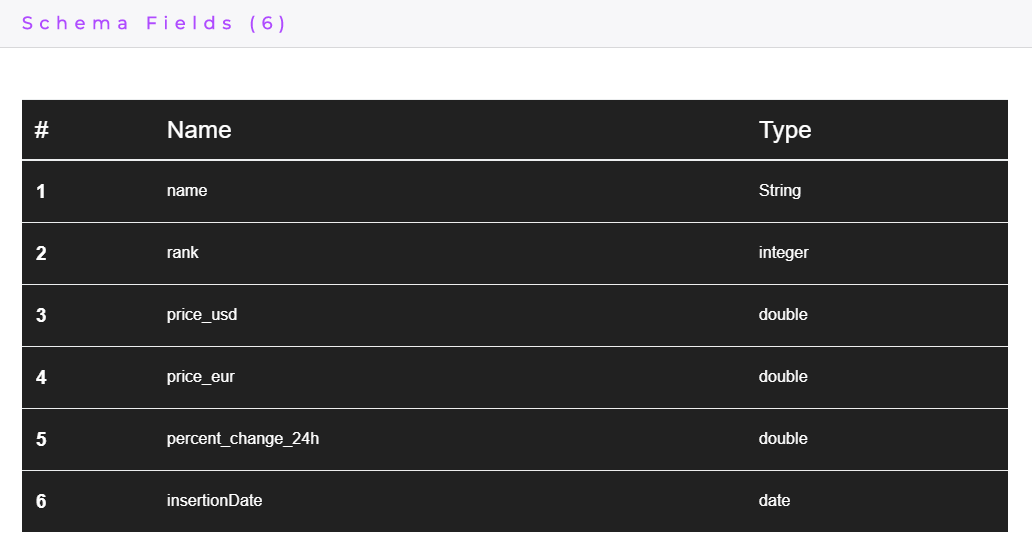
\includegraphics[width=\textwidth,height=\textheight,keepaspectratio]{iris-schema-fields}
\end{center}
A screenshot of the schema fields belonging to the Node.js schema in Iris.
\end{tcolorbox}
\caption{Node.js schema fields in Iris.}
\end{figure}

\paragraph{Data Source Endpoint}
Iris now displays the unique endpoint associated with a data source when you click on the schema in Iris. This allows a user to see what address their data source must use as well as test out the endpoint before committing to writing a data source that uses the endpoint.

\begin{figure}[H]
\begin{tcolorbox}
\begin{center}
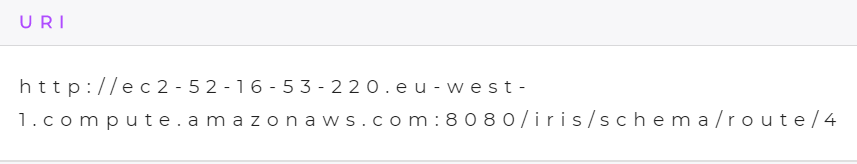
\includegraphics[width=\textwidth,height=\textheight,keepaspectratio]{iris-schema-endpoint}
\end{center}
A screenshot of the MySQL data source endpoint in Iris.
\end{tcolorbox}
\caption{MySQL data source endpoint in Iris.}
\end{figure}

\paragraph{Expected JSON}
Iris now displays the expected JSON object from the data source as well as the data types that are associated with each key in the object. This aids users when they are writing code for data sources as they can refer back to Iris to see what format their JSON object needs to conform to.

\begin{figure}[H]
\begin{tcolorbox}
\begin{center}
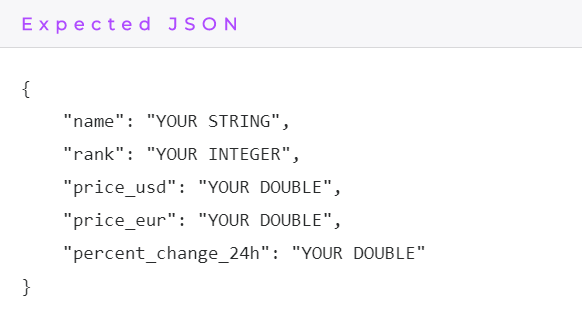
\includegraphics[width=\textwidth,height=\textheight,keepaspectratio]{iris-schema-expected-json}
\end{center}
A screenshot of the expected JSON for the Raspberry Pi data source in Iris.
\end{tcolorbox}
\caption{Expected JSON for Raspberry Pi data source.}
\end{figure}

\paragraph{Transformation/Rule Script editor}
Due to Iris' ability to allow users to write transformation scripts that run on incoming data which is discussed in \cref{para:rule:executor:backend}, a code editor was embedded into Iris. The code editor being used is the `Ace' code editor with Groovy syntax highlighting which aims to aid the user in writing small transformation scripts.

\begin{figure}[H]
\begin{tcolorbox}
\begin{center}
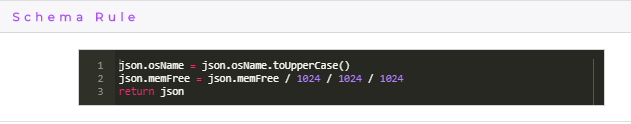
\includegraphics[width=\textwidth,height=\textheight,keepaspectratio]{node-transformation-script}
\end{center}
A screenshot of the Transformation Rule script on the Node.js schema written using the `Ace' code editor.
\end{tcolorbox}
\caption{Node.js Transformation Rule script}
\label{fig:rule:executor}
\end{figure}

More information on the `Ace' code editor can be found here \url{https://ace.c9.io/}

\paragraph{Schema Overview}
The following section ties together the previous front end sections and shows what an entire schema looks like inside Iris in a single image.

\begin{figure}[H]
\begin{tcolorbox}
\begin{center}
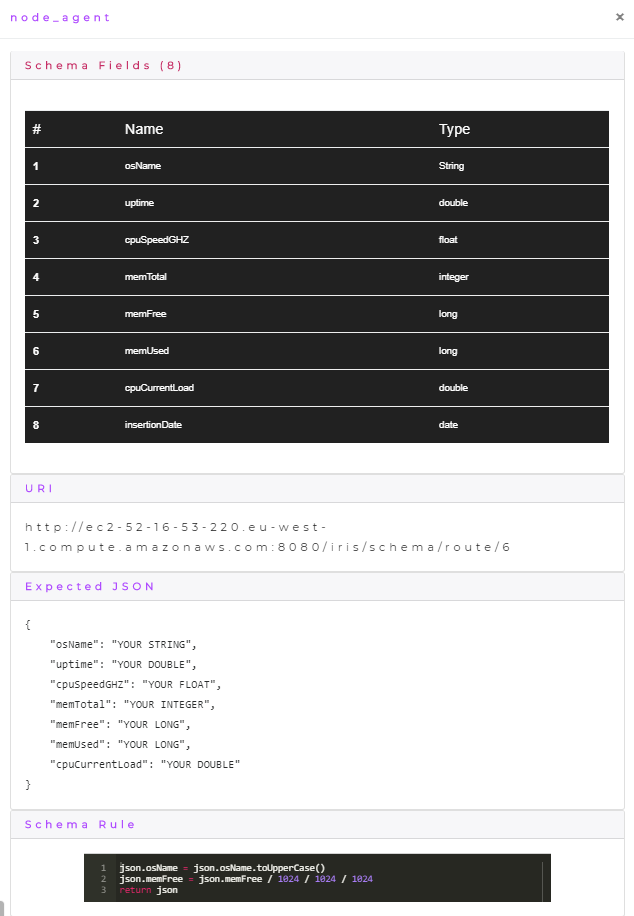
\includegraphics[width=0.8\textwidth,height=0.8\textheight]{iris-node-schema}
\end{center}
A screenshot of the Node.js agent schema in Iris.
\end{tcolorbox}
\caption{Node.js agent schema in Iris.}
\end{figure}

\subsubsection{Backend}
This section will discuss the improvements made to the backend of Iris in regards to the Schema section.

\paragraph{Transformation/Rule Script Execution}
\label{para:rule:executor:backend}
In the semester 1 report it was briefly discussed that Iris would allow users to write their own scripts inside Iris to allow a user to modify incoming data, which would avoid a user having to redeploy their data source to make a small change to the data they are pushing ot Iris. A user would mainly use this feature for formatting dates, strings and numerical values before it is inserted into Elasticsearch and rendered on the user's dashboard. This feature is now fully supported in Iris and an image of a transformation script can be found in \cref{fig:rule:executor}

\paragraph{Data Source Endpoint Retrieval}
Iris now accepts `POST' requests to the endpoint \url{$SERVER_BASE/schema/getAgentUrl} and expects a JSON body with the request like the following:

\begin{figure}[H]
\begin{tcolorbox}
\begin{minted}{json}
{
    "name": "someSchemaName"
}
\end{minted}
\end{tcolorbox}
\caption{SchemaController getAgentUrl endpoint JSON payload.}
\end{figure}
Assuming the user is authenticated, Iris will look for a Schema matching this name and return the unique endpoint for this schema. The advantage of this is that a user may create a schema and not be satisfied with it. The user may then decide to delete the schema and create a new schema using the same name with extra attributes attached to it. The issue here is that Iris will give the new schema a new url different from the previous schema. This now means a user must go back to their agent code and change a hardcoded url to a new url and then redeploy the agent. However if a user writes their code to take advantage of the `getAgentUrl' endpoint in Iris, they will be able to dynamically obtain a new unique endpoint for the new schema as long as the schema name stays the same. This means there is no need to redeploy the agent with a new url as it is obtained dynamically from Iris.

\begin{figure}[H]
\begin{tcolorbox}
\begin{center}
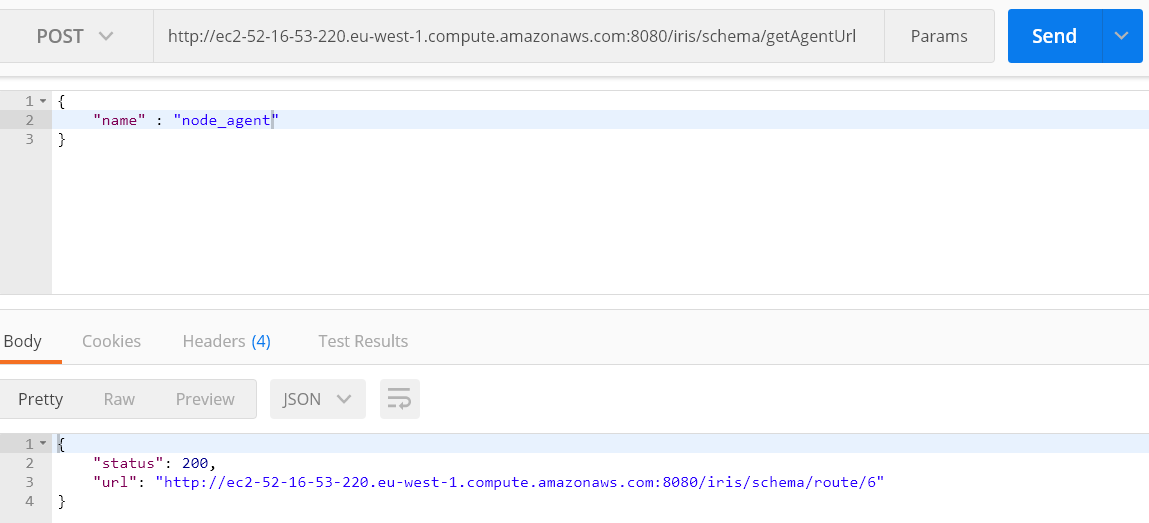
\includegraphics[width=\textwidth,height=\textheight,keepaspectratio]{iris-get-agent-url}
\end{center}
A screenshot of the `getAgentUrl' endpoint being used in Postman to retrieve the Node.js agent's endpoint.
\end{tcolorbox}
\caption{SchemaController `getAgentUrl' endpoint in Postman.}
\end{figure}

\paragraph{Timestamping Data}
Iris now puts a timestamp on all incoming data before it is inserted into Elasticsearch. The timestamp is added as a schema field called `insertionDate' under the schema to which the data belongs. This field is used in the background of the Aggregation Builder in Iris and will be discussed in that section.

\subsection{Dashboards}
In the semester 1 report the javascript libraries for building Iris' dashboard system were selected and tested on a very small scale. The design for implementing the dashboard and updating the charts in realtime have remained the same throughout the implementation this semester. The dashboard system features and implementation will be discussed in terms of frontend and backend logic in the following sections. A brief overview of how the data flows into the dashboard will also be discussed.
 
\subsubsection{Frontend}
This section will discuss the major factors of the frontend of the Iris dashboard system.

\paragraph{Gridstack.js}
Gridstack.js was briefly discussed in the semester 1 report as being the library that was selected to aid in the dashboard creation. In semester 1 the library was and it's api was researched to ensure it supported the features Iris required.

Due to the extensive research on the library in semester 1 and the active github support from the Gridstack.js developers there was no major issues during the implementation phase in semester 2. Gridstack.js was used to contain the contents of a dashboard in a grid format. Whenever a chart is created for a dashboard a new widget is created containing the chart and added to the Gridstack grid. This widget automatically becomes resizeable, draggable and serializeable.

The logic used to format the Gridstack grid into a serializeable object was retrieved from the Gridstack.js serialize demo, which can be found here \url{https://dsmorse.github.io/gridster.js/demos/serialize.html}. Using the basic structure supplied by the Gridstack.js developers, Iris' client code expanded upon this functionality to support chart types and aggregation objects to be included in the serialized data.
\begin{figure}[H]
\centering
\begin{tcolorbox}
    \begin{subfigure}{\textwidth}
        \begin{tcolorbox}
        \centering
        \begin{minted}[breaklines,frame=lines]{javascript}
        this.serializedData = _.map($('.grid-stack > .grid-stack-item:visible'), function (el) {
            el = $(el);
            var node = el.data('_gridstack_node');
            return {
                x: node.x,
                y: node.y,
                width: node.width,
                height: node.height
            };
        }, this);
        \end{minted}
        \caption{Gridstack.js Developer's Serialization logic}
    \end{tcolorbox}
    \end{subfigure}%
    \newline
    \begin{subfigure}{\textwidth}
        \begin{tcolorbox}
        \centering
        \begin{minted}[breaklines,frame=lines]{javascript}
        serializedData = _.map($('.grid-stack > .grid-stack-item:visible'), function (el) {
        el = $(el);
        var node = el.data('_gridstack_node');
        var widgetInfo = el.data();
        return {
            x: node.x,
            y: node.y,
            width: node.width,
            height: node.height,
            id: node.el[0].id,
            schemaId: widgetInfo.schemaid,
            chartName: widgetInfo.chartname,
            chartType: widgetInfo.charttype,
            data: JSON.parse(localStorage.getItem(node.el[0].id))
        };
    }, this);
        \end{minted}
        \caption{Iris Dashboard Serialization logic}
    \end{tcolorbox}
    \end{subfigure}

\end{tcolorbox}
\caption{Iris extension of Gridstack.js Serialization}
\end{figure}
One main issue that was found with the Gridstack library is that if a chart contains no data it does not scale the chart correctly and makes the chart overflow to one side making it appear compact. Unfortunately this issue is not consistent and as a result was not fixed. Currently the only fix is to click on the resizeable handles of a widget and the chart then scales correctly.

For a basic demo of Gridstack.js refer to this url \url{http://gridstackjs.com/demo/}
\paragraph{Billboard.js}
In the semester 1 report Billboard.js was selected as the charting library that Iris would use in its dashboard system. Billboard.js was researched and tested heavily in semester 1 but was not implemented within Iris until semester 2.

Implementing Billboard.js into Iris was relatively straight forward because of the testing done in semester 1, the only difference was that the Billboard.js charts were now going to be dynamically added to a grid and contained within a Gridstack.js widget. This was not difficult as it was simply an extra parent container to be added around the chart element.
The chart type support will be discussed in \cref{para:charts:fontend} and the chart subscriptions will be discussed in \cref{para:charts:subs:frontend}.

For examples of charts created with Billboard.js see this url \url{https://naver.github.io/billboard.js/demo/}

\paragraph{Chart Types}
\label{para:charts:fontend}
% discuss all the chart types supported
Iris supports the following chart types:
\begin{itemize}
    \item Bar Chart
    \item Bubble Chart
    \item Pie Chart
    \item Line Chart
    \item State Disc Chart (A chart used for monitoring state based data)
    %TODO ADD PIC OF EACH CHART
\end{itemize}
\paragraph{Chart Subscriptions}
\label{para:charts:subs:frontend}
The design for how Iris would handle sending incoming data to the correct charts was created and documented in the semester 1 report. However the design was not tested and implemented until semester 2. The libraries chosen in semester 1 for web socket functionality remained the same. Iris uses the Grails Web Socket plugin to add socket communication between dashboard charts and the server, allowing charts to subscribe to incoming data. 

Each client chart on an Iris dashboard subscribes to messages from the server on a unique socket endpoint, which ensures the correct data gets sent to the correct chart. This design was discussed in the semester 1 report and remained the same for the implementation of the chart subscription logic in Iris.

For more information on he Grails 3 `grails-spring-websocket' plugin refer to \url{https://github.com/zyro23/grails-spring-websocket}.
\begin{figure}[H]
\begin{tcolorbox}
\begin{minted}[breaklines]{javascript}
function setChartSubscription(subscriptionId, chart, chartType, schemaId){
    //this subscription is for updates being sent to the chart
    client.subscribe("/topic/" + schemaId + "/" + chartType + "/" + subscriptionId, function(message) {
        var parsedMsg = JSON.parse(message.body);
        //update the chart
        if(chartType != chartTypes.StateDisc){  //REGULAR CHARTS
            updateBasicCharts(chart, parsedMsg);
        }else{  //STATE BASED CHARTS
            updateStateDiscChart(chart, parsedMsg);
        }
    });

    //this subscription is for initial loading data for the chart
    client.subscribe("/topic/load/" + schemaId + "/" + chartType + "/" + subscriptionId, function(message){
        var parsedMsg = JSON.parse(message.body);
    // update the chart
        chart.instance.load({
            columns: parsedMsg.data.columns,
            length: 0
        });
    });
}
\end{minted}
\end{tcolorbox}
\caption{Iris Client Side Chart Subscription logic.}
\end{figure}
\paragraph{Downloadable Chart Data}
Iris now supports the ability to download a JSON file consisting of the current data being displayed on the chart that was picked to be downloaded. Each chart on the dashboard has this functionality. This functionality was built by using the Billboard.js api and retrieving the chart data, and adding custom logic to put that data into a file to be downloaded upon request.
\begin{figure}[H]
\begin{tcolorbox}
\begin{center}
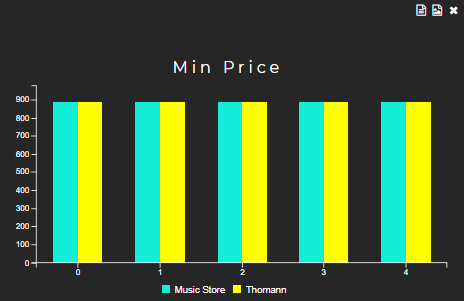
\includegraphics[width=\textwidth,height=\textheight,keepaspectratio]{iris-downloaded-chart}
\end{center}
A screenshot of a downloadable chart in Iris, taken from the `selenium agent' dashboard in Iris. The file icon in the top right is clicked to start the download.
\end{tcolorbox}
\caption{Downloadable Chart Example}
\label{fig:downloaded:chart}
\end{figure}

\begin{figure}[H]
\begin{tcolorbox}
\begin{minted}[breaklines]{json}
[{"id":"Music Store","id_org":"Music Store","values":[{"x":0,"value":888,"id":"Music Store","index":0},{"x":1,"value":888,"id":"Music Store","index":1,"name":"Music Store"},{"x":2,"value":888,"id":"Music Store","index":2},{"x":3,"value":888,"id":"Music Store","index":3},{"x":4,"value":888,"id":"Music Store","index":4}]},{"id":"Thomann","id_org":"Thomann",
"values":[{"x":0,"value":888,"id":"Thomann","index":0},
{"x":1,"value":888,"id":"Thomann","index":1,"name":"Thomann"},
{"x":2,"value":888,"id":"Thomann","index":2},
{"x":3,"value":888,"id":"Thomann","index":3},
{"x":4,"value":888,"id":"Thomann","index":4}]}]
\end{minted}
\end{tcolorbox}
\caption{JSON file data downloaded from a chart on the  `selenium agent' dashboard as shown in \cref{fig:downloaded:chart}.}
\end{figure}

\paragraph{Revision History}
Iris now supports revision history for all dashboards, meaning a user can navigate between previous versions of a dashboard by simply using a select box on the dashboard page which allows the user select the revision they wish to view.
\begin{figure}[H]
\begin{tcolorbox}
\begin{center}
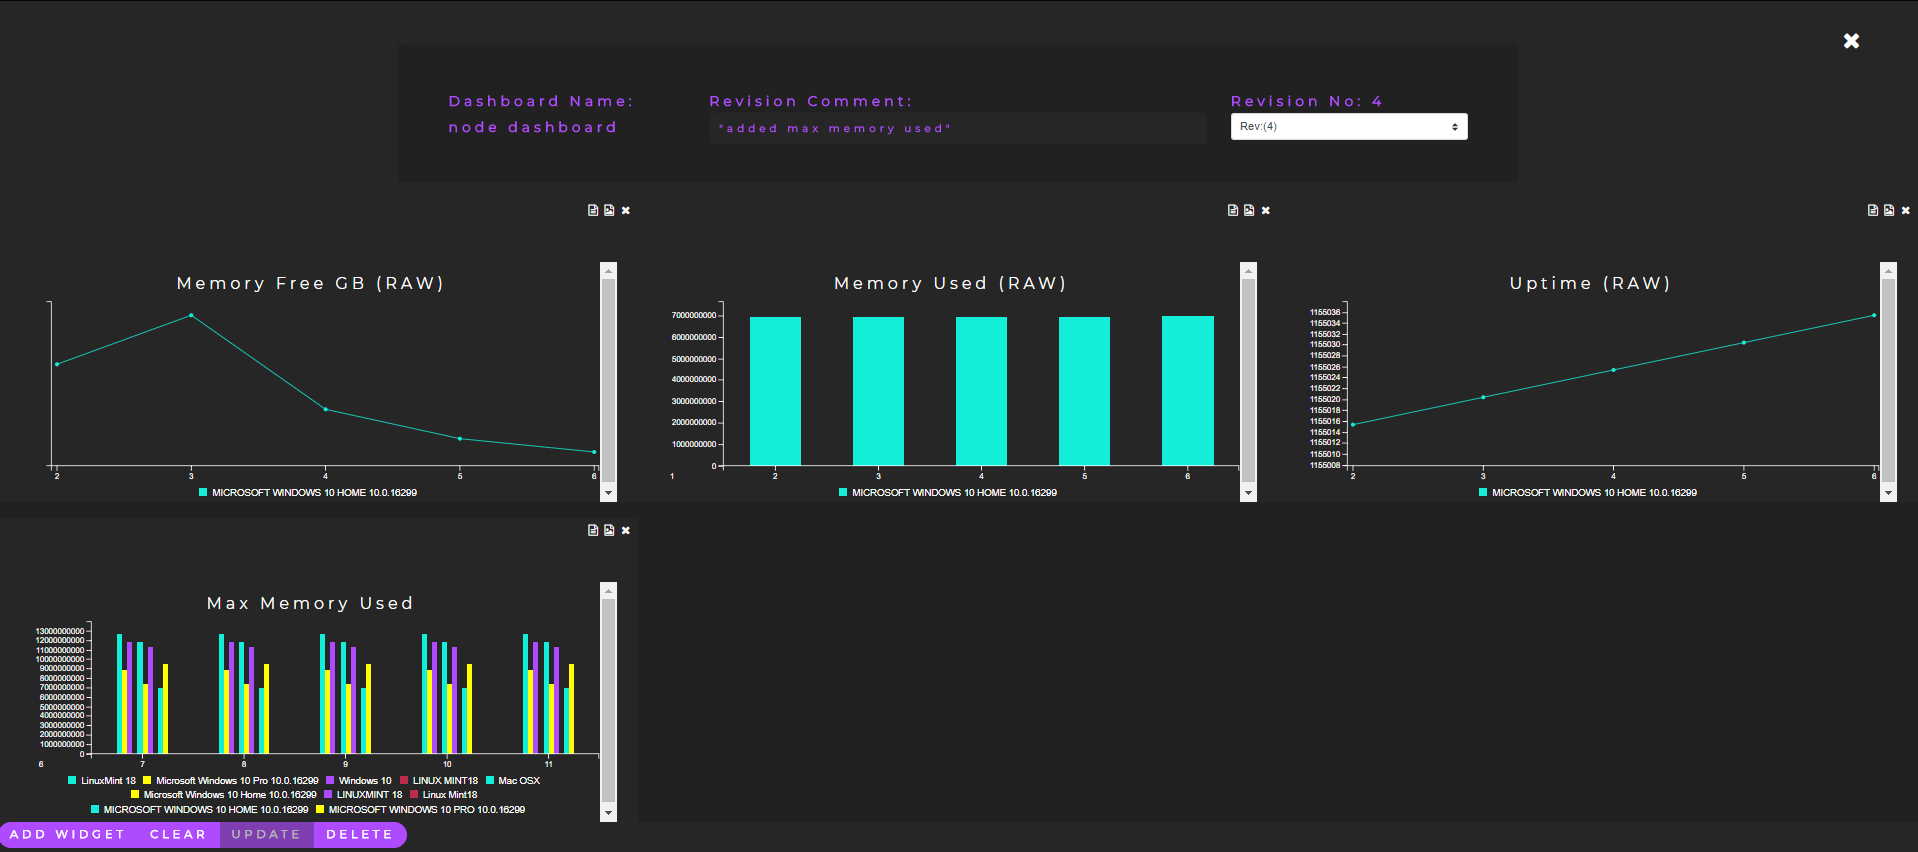
\includegraphics[width=\textwidth,height=\textheight,keepaspectratio]{iris-node-dash-rev-1}
\end{center}
A screenshot of the Node.js dashboard in Iris capturing its fourth revision.
\end{tcolorbox}
\caption{Node.js Dashboard Revision No. 4}
\label{fig:dash:rev:4}
\end{figure}
\begin{figure}[H]
\begin{tcolorbox}
\begin{center}
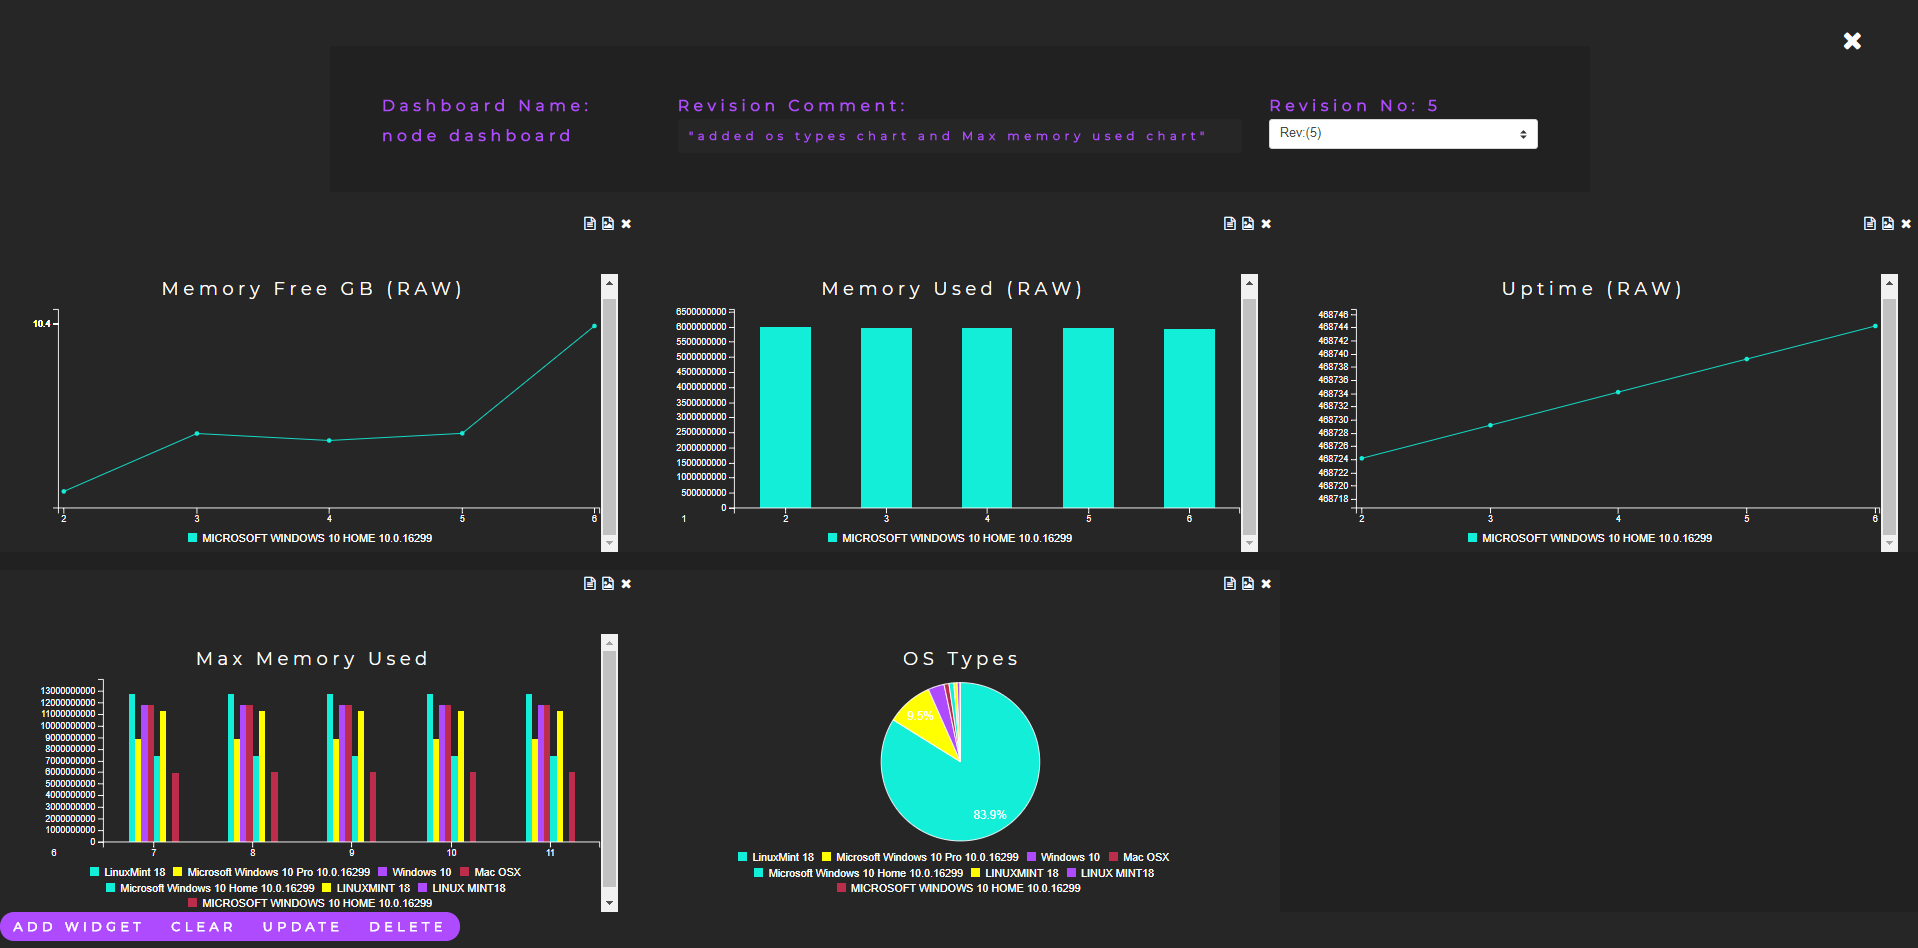
\includegraphics[width=\textwidth,height=\textheight,keepaspectratio]{iris-node-agent-dashboard}
\end{center}
A screenshot of the Node.js dashboard in Iris capturing its fifth revision. Note the extra chart `OS Types' that was added to this revision compared to the fourth revision show in \cref{fig:dash:rev:4}.
\end{tcolorbox}
\caption{Node.js Dashboard Revision No. 5}
\end{figure}

\subsubsection{Backend}
This section will focus on the backend implementation of the Iris dashboard system.
\paragraph{Chart Types}
The Iris chart types are handled by using enums in Iris. This allows for the code in Iris to be easily expanded upon when a new chart type is needed, and the use of enums allows for more readable code when dealing with different types of charts.

\begin{figure}[H]
\begin{tcolorbox}
\begin{minted}[breaklines]{groovy}
enum ChartType {

    BAR("Bar"),
    BUBBLE("Bubble"),
    PIE("Pie"),
    LINE("Line"),
    STATE_LIST("StateList"),
    STATE_DISC("StateDisc");

    private String value;

    private ChartType(String value){
        this.value = value;
    }

    String getValue(){ return this.value; }
}
\end{minted}
\end{tcolorbox}
\caption{ChartType.groovy enum from Iris.}
\end{figure}
Due to Iris supporting different chart types as well as different types of data, each chart has optional attributes such as an Elasticsearch aggregation if the user created the chart using an aggregation, and a raw attribute in the case of a user wishing to just send raw data to the chart and not have Elasticsearch perform any aggregations over the incoming data.
\begin{figure}[H]
\begin{tcolorbox}
\begin{minted}[breaklines]{groovy}
class Chart {

    String name
    String chartType
    String subscriptionId
    Aggregation aggregation
    IrisSchema schema
    boolean isRaw = false
    boolean archived = false

    static constraints = {
        name(nullable: false, blank: false)
        chartType(nullable: false, inList: ChartType.values()*.getValue())
        aggregation(nullable: false)
        schema(nullable: false)
        archived(nullable: true)
        subscriptionId(nullable: true)
        isRaw(nullable: true)
    }

    static belongsTo = [grid: Grid]
}
\end{minted}
\end{tcolorbox}
\caption{Chart.groovy domain for representing Charts in Iris.}
\end{figure}

\paragraph{Chart Subscriptions}
When data enters Iris, Iris uses the chart type to figure out how a chart should be updated. For all charts the flow of data is the same, a data source will send data to Iris and Iris will send the data to the chart using a Grails Service which which comes as part of the `grails-spring-websocket' plugin. If a chart is marked as raw or of type `State Disc' then the data being sent to the chart is not modified, if a chart instance has an Elasticsearch aggregation attached to it the aggregation is executed in Elasticsearch and the result is parsed and formatted to suit the chart type and then sent to the chart to be updated on the frontend.

\paragraph{Serilization}
Iris serializes Dashboard domains through composition. Each Dashboard domain has a Grid domain object which stores the entire dashboard in JSON. This means that serializing and loading dashboards is simply done with a string of JSON. This JSON is passed to the frontend where it is parsed by the client to create the dashboard.

Due to Iris storing the dashboard grid as a JSON string, it allows for Iris to extend its dashboard system in the future by allowing users to build dashboards offline or locally and upload a JSON file which represents their dashboard. Iris will be able to save and load the dashboard as long as the user conforms to the existing dashboard JSON structure which is in place.

\paragraph{Revision History}
Iris supports revision history for its dashboard system. When a dashboard is initially created Iris will create a new Revision domain object to associate with the dashboard. This revision object has a unique id which is referred to as the `revisionId', this id is specific to each dashboard. Along with the revision id, a revision number is also stored, meaning all revisions specific to a dashboard have the same revision id and different revision numbers. Whenever a dashboard is updated and the changes are committed, Iris will create a new revision for the dashboard by coping the revision id of the most recent revision and then incrementing the revision number of the most recent revision. This results in a brand new revision being created. When a dashboard is rendered on the frontend of Iris the backend sends down all the revisions associated with the dashboard which allows the user to select what version of the dashboard they wish to view.

\begin{figure}[H]
\begin{tcolorbox}
\begin{center}
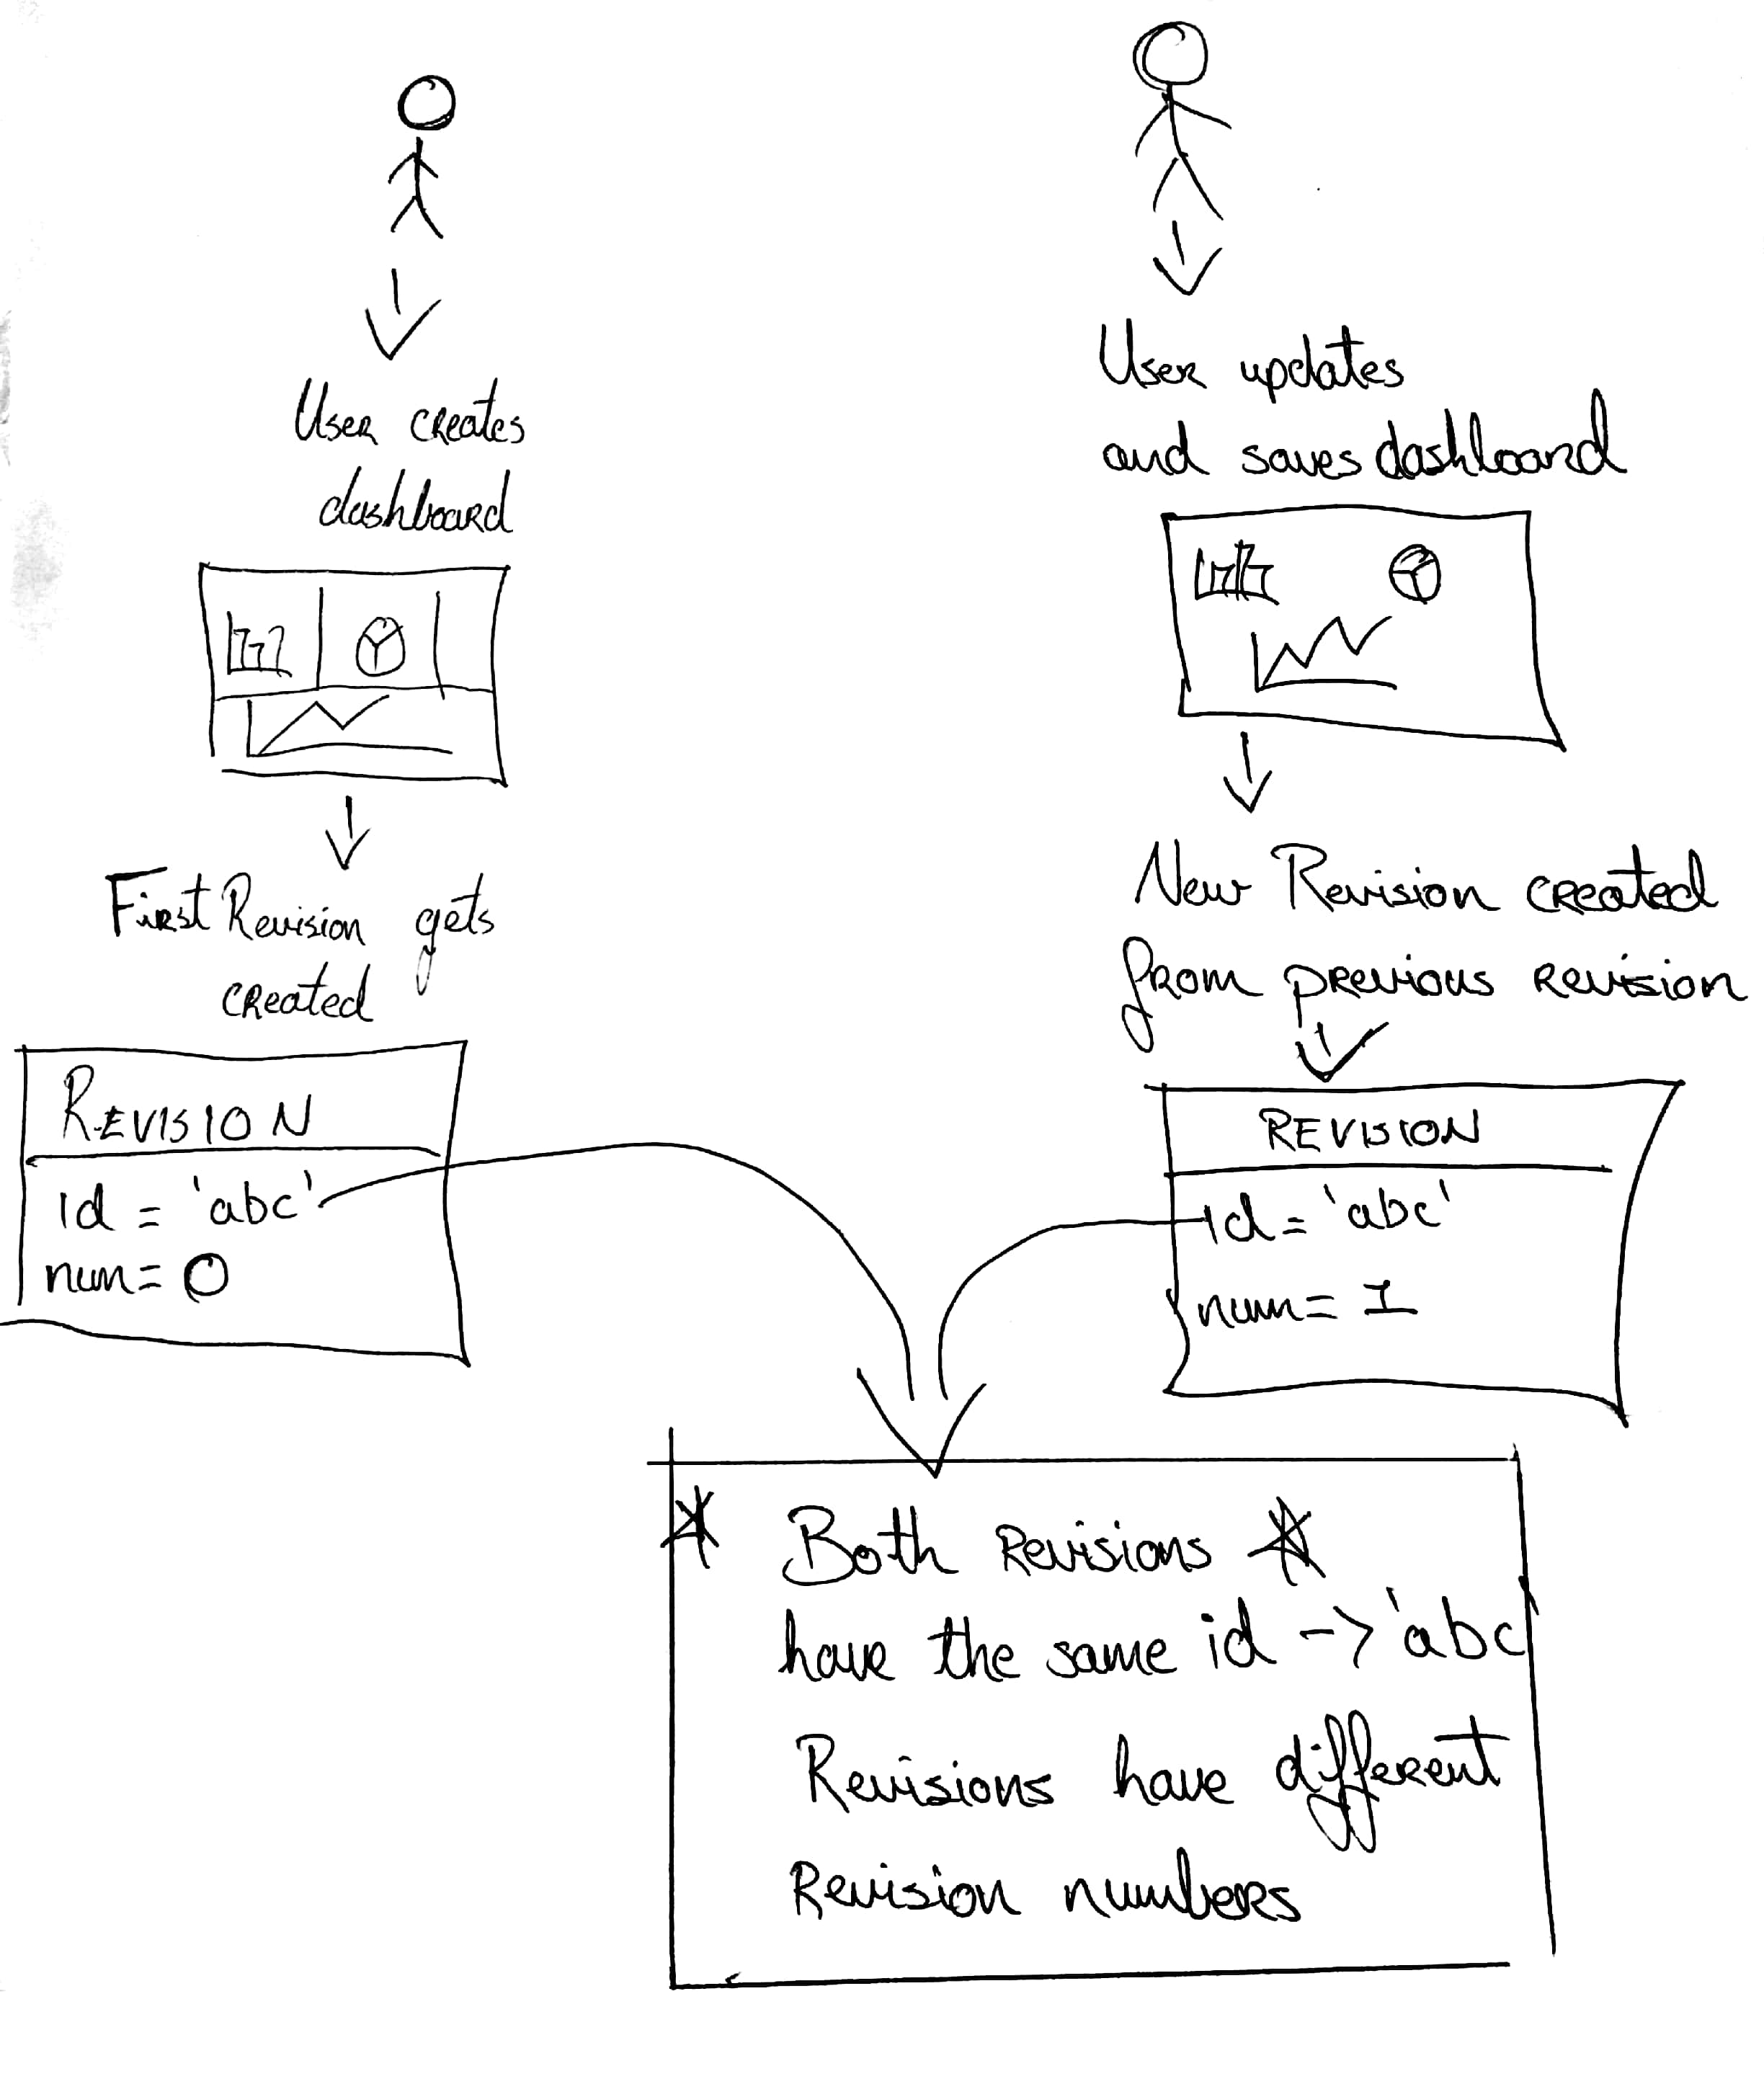
\includegraphics[width=\textwidth,height=\textheight,keepaspectratio]{iris-dash-revision}
\end{center}
An image showing how the revision history of dashboards works in Iris.
\end{tcolorbox}
\caption{Iris Dashboard Revision Diagram.}
\end{figure}

\paragraph{Scalability}
A big concern with Iris in the beginning was to see how scalable the dashboard system would be if a lot of data was being sent to Iris. In an effort to make the dashboard system more efficient Iris dashboards have a boolean attribute called `isRendering'. When a dashboard is being viewed by a user the backend toggles the `isRendering' state of the dashboard to true, this is switched to false once a dashboard is no longer being viewed. The reason for this is to prevent data being modified and formatted for a dashboard which is not being rendered to the user. By having this state attached to a dashboard, a dashboard will only be sent updates if it is being viewed by a user, otherwise the data will simply be entered into Elasticsearch and no more code will be executed. This makes the dashboards much more efficient and scalable as Iris is only dealing with dashboards that are being viewed.

\begin{figure}[H]
\begin{tcolorbox}
\begin{center}
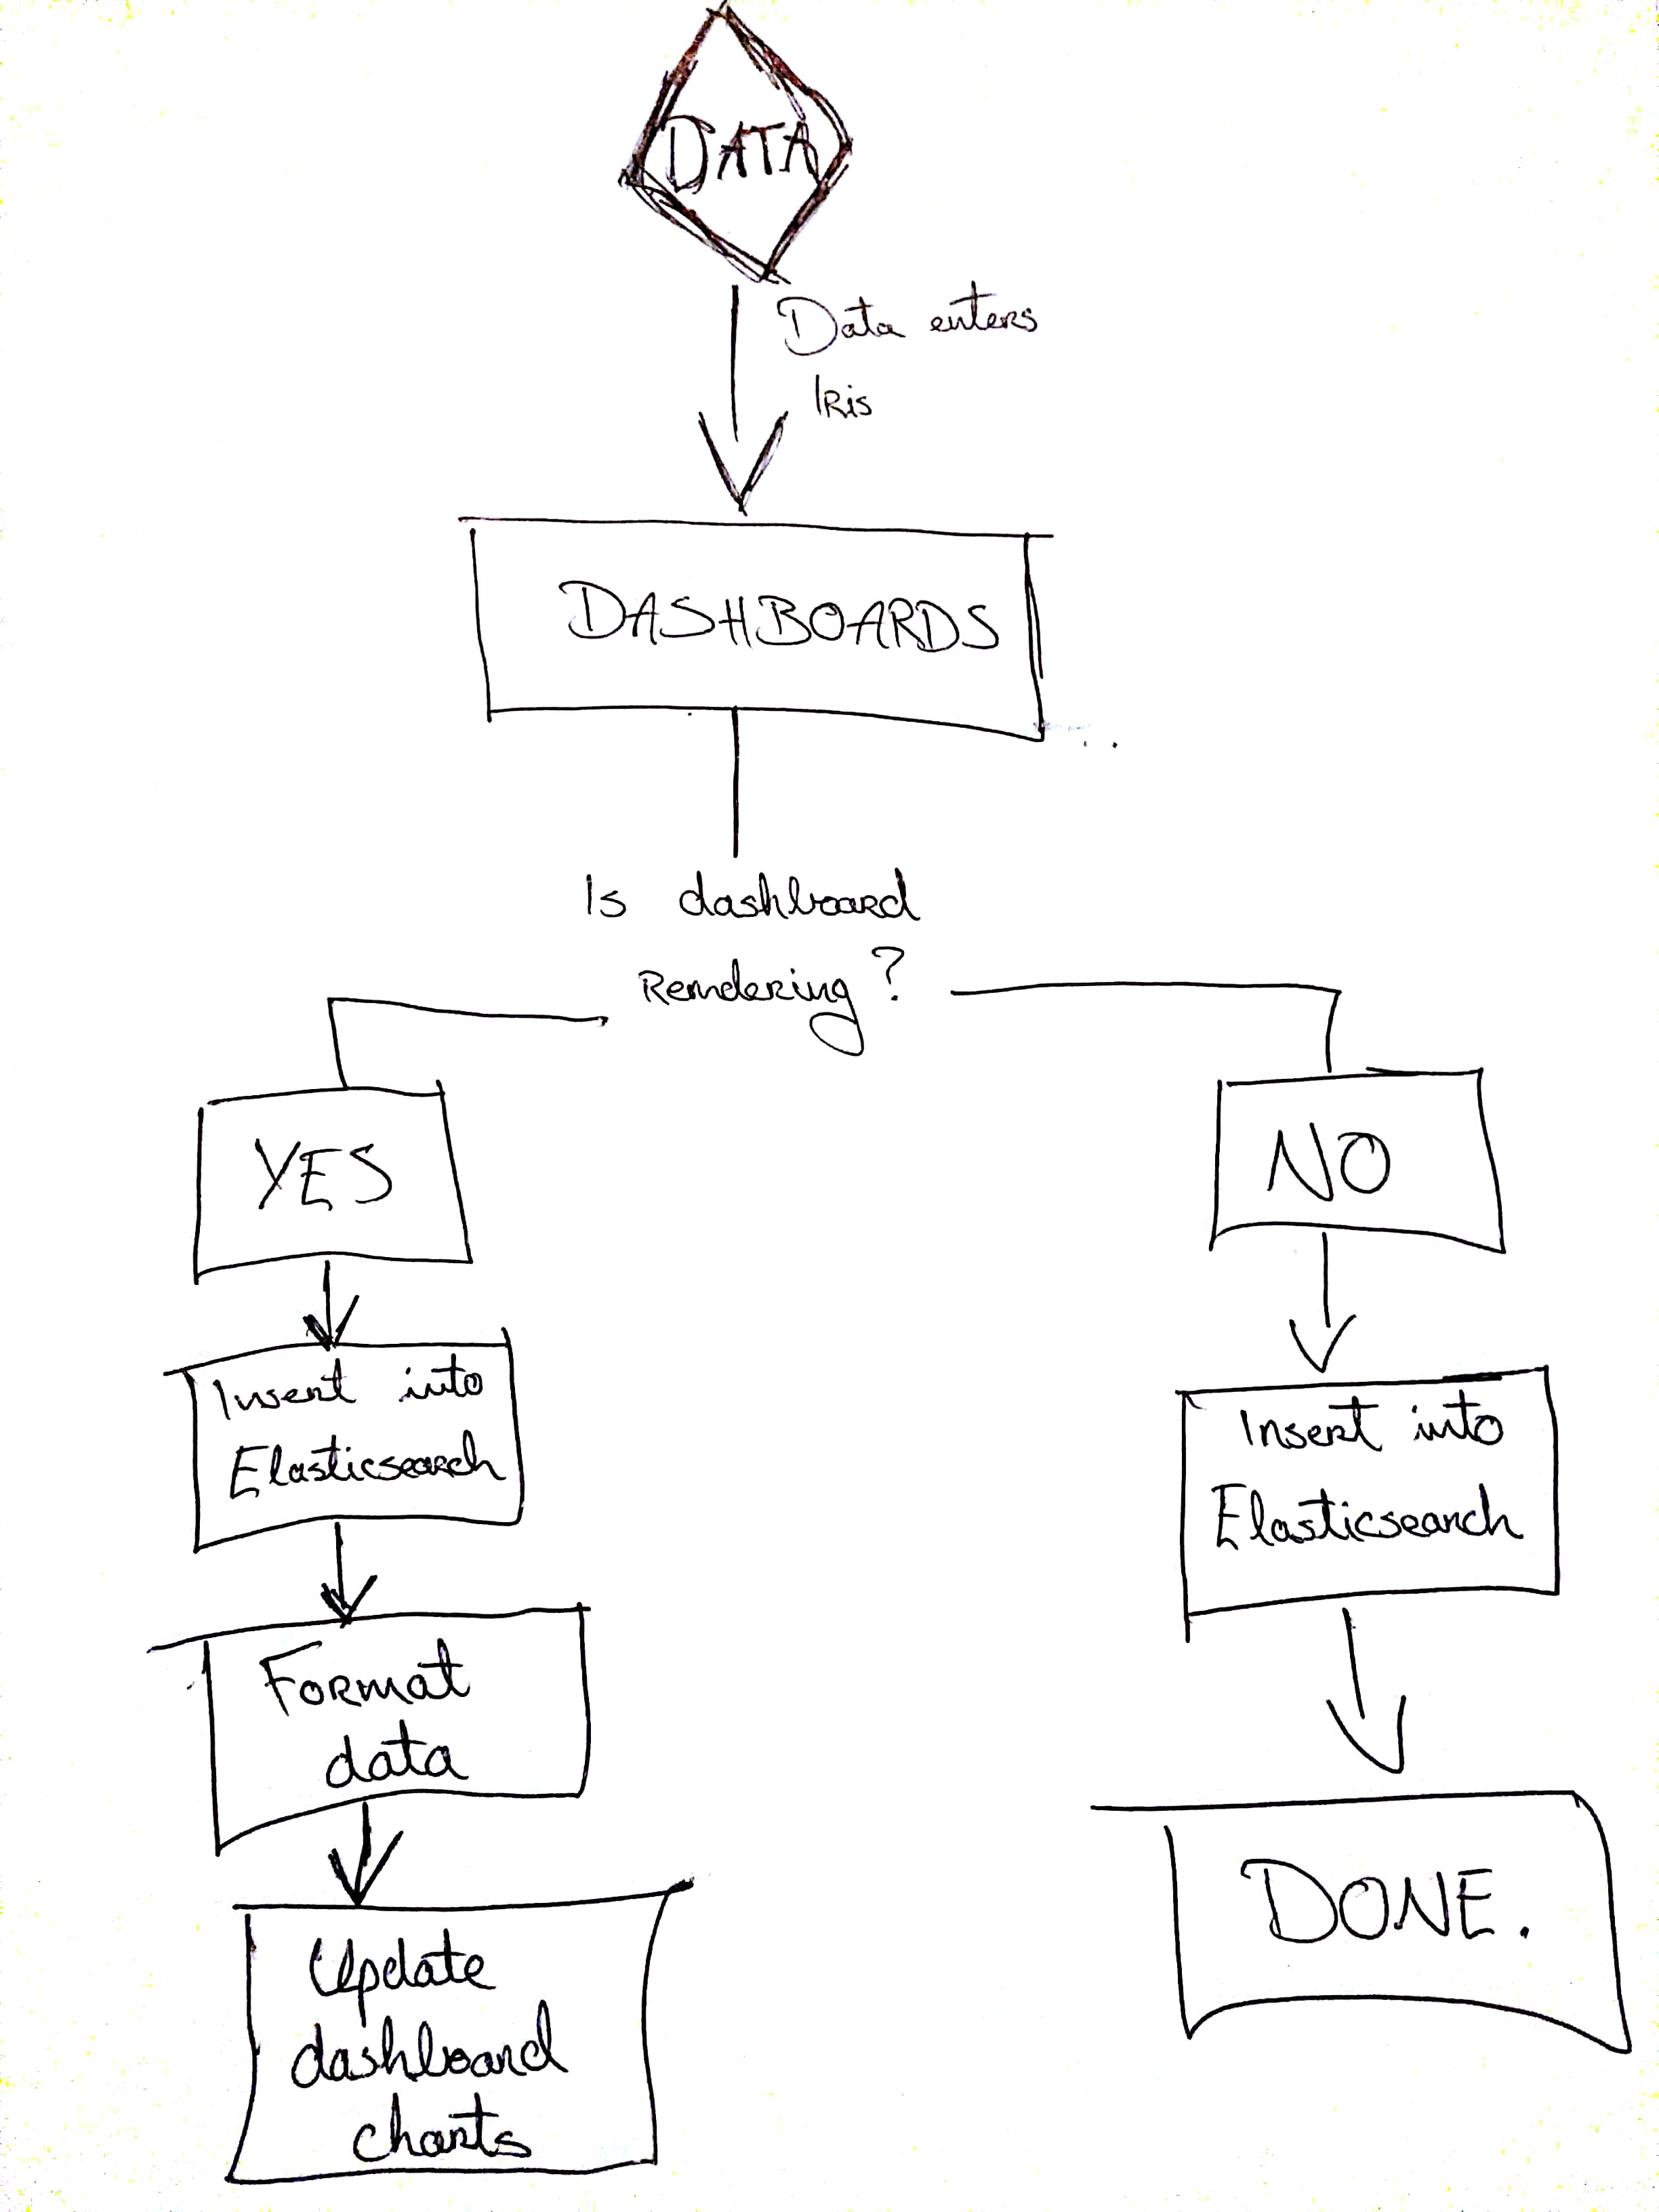
\includegraphics[width=\textwidth,height=\textheight,keepaspectratio]{iris-dash-scalability}
\end{center}
A flow chart showing how Iris handles dashboards that are rendering versus dashboards that are not rendering.
\end{tcolorbox}
\caption{Iris Dashboard Scalability.}
\end{figure}

\subsection{Aggregation Builder}
%basics of this were implemented in semester 1
\subsubsection{Aggregation Types}
% List all possible aggregations you can test
%Talk about being able to aggregate over all data in elasticsearch, not advisable for dashboards if data is large
%that it supports moving numerical data like moving average, max, min etc.... which aggregates a number of the most recent documents
\subsubsection{Aggregation Builder Preview}
%talk about how the user can see the json being built as they nest aggregations

\subsection{Security}
% talk about the addition of security in iris

\subsubsection{Spring Security Core}
%spring security core was used to generate a user, role and user role and secure the app from unauthenticated users
\subsubsection{Spring Security REST Plugin}
%talk about securing the rest endpoints with spring security rest, jwt and login api

\subsubsection{Testing Security}
%tested using postman

\subsubsection{Data Source Adaptation}
%now use login api to get authenticated and given a token, they then send this token with every request to iris


\section{Data Sources}

A DataSource can be any process that generates data and pushes it to Iris. %In \Cref{s:Implementation:DataSource}
and number of examples of data sources are discussed. THe Implementation details of these data sources is not covered in detail because they are not germane to the this project and follow well know patterns.

\chapter{Deployment, Testing and Evaluation}

\section{Deployment}
\subsection{AWS}
\subsection{Jetty}
\subsection{Gradle}
\subsection{WAR}
\subsection{MySQL GORM Mapper}

\section{Testing and Evaluation --- Data Sources}
\subsection{Introduction}
A number of data source have been implemented to demonstrate the flexibility of Iris and to test the aggregation. Each
of the following sections describe a data source and its unique features.

\subsection{Android App}
\subsubsection{Description}
The android application demonstrates how Iris handles state based data. The application is very simple, but demonstrates how simple it is to monitor an application's state through Iris. The application is simply a screen consisting of six tiles. Each tile represents a different state, each state has three colours and three numerical values linked to the states and colours. The android application allows the user to change the states of these tiles, which then changes the state of the tile colour and value. When a user is satisfied with the states they wish to send to Iris they simply tap the screen. This results in a JSON object being sent to Iris consisting of the current numerical value for each state tile i.e the current state of the tiles.
%Iris Android app screenshot
\begin{figure}[H]
\begin{tcolorbox}
\begin{center}
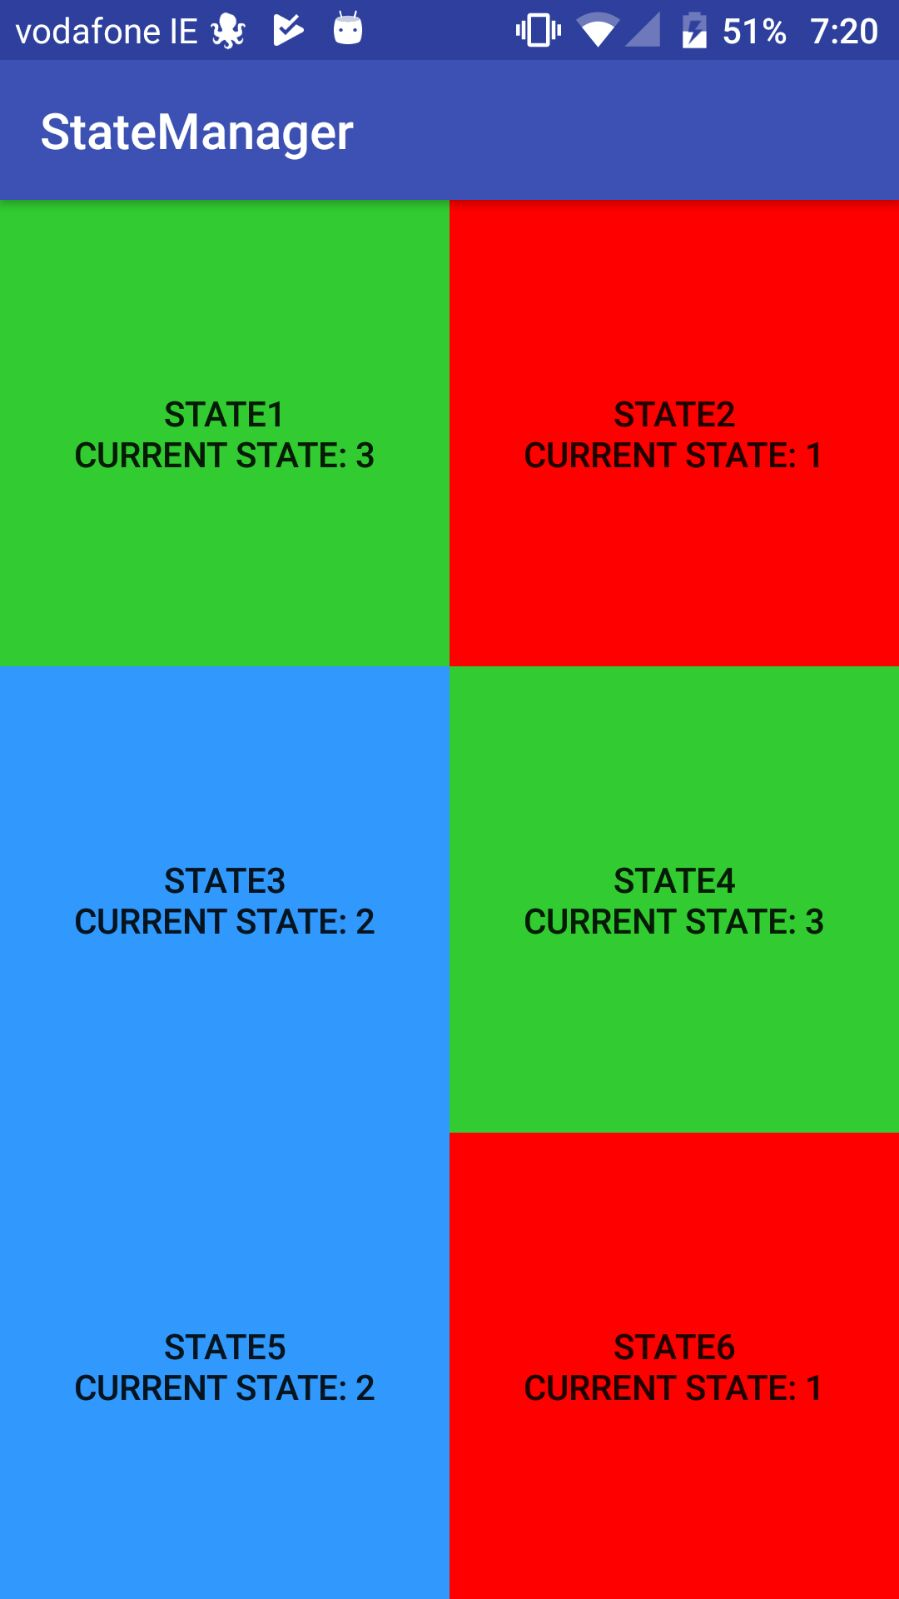
\includegraphics[width=0.7\textwidth,height=0.7\textheight]{android-agent}
\end{center}
A screenshot of the android agent and its state based tiles. Each of the tiles on the screen holds a state, the states are as follows:
\begin{itemize}
    \item State 1 - Values:(1, 2, 3), Colours:(Red, Blue, Green)
    \item State 2 - Values:(1, 2, 3), Colours:(Red, Blue, Green) 
    \item State 3 - Values:(1, 2, 3), Colours:(Red, Blue, Green) 
    \item State 4 - Values:(1, 2, 3), Colours:(Red, Blue, Green) 
    \item State 5 - Values:(1, 2, 3), Colours:(Red, Blue, Green) 
    \item State 6 - Values:(1, 2, 3), Colours:(Red, Blue, Green) 
\end{itemize}
\end{tcolorbox}
\caption{Android agent for Iris.}
\end{figure}

\subsubsection{Linkage with Iris}
The android application is linked to Iris through a unique REST endpoint specific to the android agent schema. All of the data being sent from the android application is sent to this endpoint. Once the data enters Iris, Iris will run through it's logic for checking for dashboards and charts associated with the schema and send the data through to the charts. 
%Add a ref to a section where you explain what iris does, so you dont have to keep repeating this for all agents
In this case the charts are state based and will update according to the state values that are given to them.

\begin{figure}[H]
\begin{tcolorbox}
\begin{center}
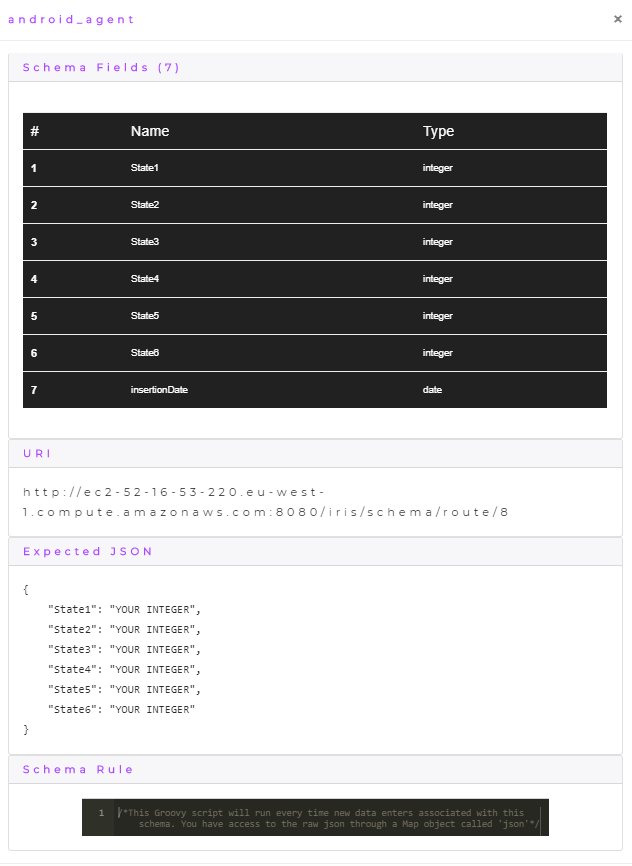
\includegraphics[width=\textwidth,height=\textheight,keepaspectratio]{iris-android-schema}
\end{center}
A screenshot of the Android agent schema in Iris.
\end{tcolorbox}
\caption{Android agent schema in Iris.}
\end{figure}

%Iris Android agent dashboard screenshot
\begin{figure}[H]
\begin{tcolorbox}
\begin{center}
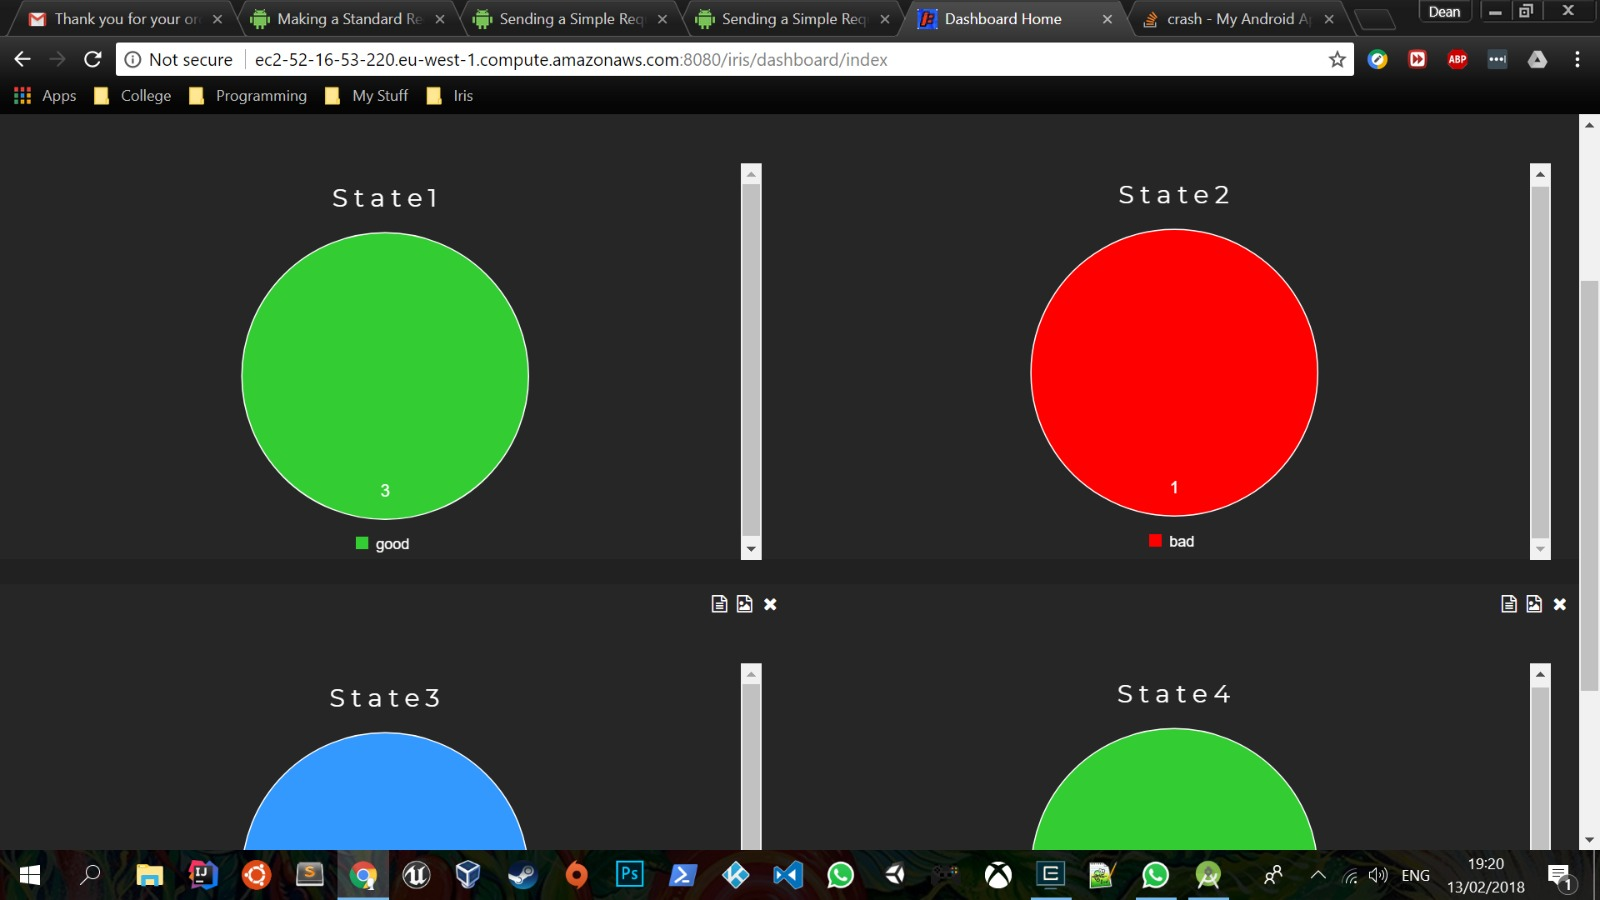
\includegraphics[width=\textwidth,height=\textheight,keepaspectratio]{iris-android-dashboard}
\end{center}
A screenshot of the android agent dashboard in Iris and its state based tiles.
\end{tcolorbox}
\caption{Android agent dashboard in Iris.}
\end{figure}

\subsection{Raspberry Pi}
The Raspberry Pi agent is used to demonstrate the plug and play ability of a Raspberry Pi combined with the versatility of Iris.

\subsubsection{Description}
The Raspberry Pi agent demonstrates how a user can use a Raspberry Pi to run a script to continuously monitor an API. In the case the Raspberry Pi monitors crypto currency exchange rates using a python script through a library called `coinmarketcap'. The python script simply retrieves the latest crypto currency data through the `coinmarketcap' library and sends the data to the corresponding `crypto\_agent' endpoint in Iris. The Raspberry Pi agent is configured to run the script every minute with crontab and is also configured to automatically sign in to the terminal. This results in a plug and play agent wherever their is a network cable available.

For more information on coinmarketcap see their site here \url{https://coinmarketcap.com/}

\subsubsection{Linkage with Iris}
The Raspberry Pi agent is linked to Iris through a unique REST endpoint specific to the Raspberry Pi agent schema. All of the data being sent from the Raspberry Pi is sent to this endpoint. Once the data enters Iris, Iris will run through it's logic for checking for dashboards and charts associated with the schema and send the data through to the charts. 
%Add a ref to a section where you explain what iris does, so you dont have to keep repeating this for all agents
In this case Iris is monitoring raw data on two charts that are monitoring the current price in euro and usd. The other charts are using Elasticsearch aggregations to monitor the min and max prices reached for currencies in both euro and usd.

%Raspberry Pi agent schema screenshot in Iris
\begin{figure}[H]
\begin{tcolorbox}
\begin{center}
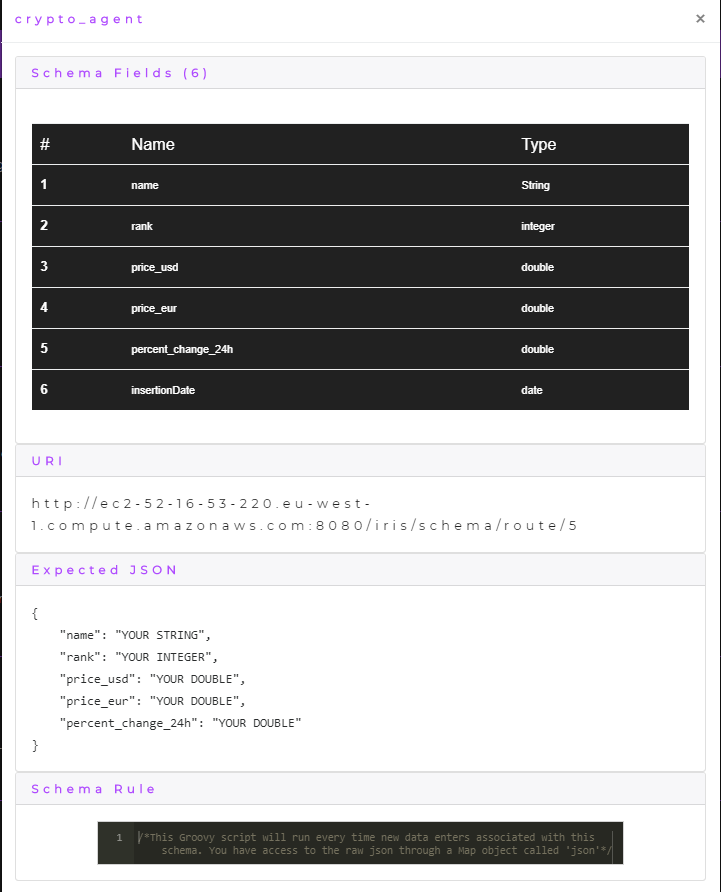
\includegraphics[width=\textwidth,height=\textheight,keepaspectratio]{iris-crypto-schema}
\end{center}
A screenshot of the Raspberry Pi agent schema in Iris.
\end{tcolorbox}
\caption{Raspberry Pi agent schema in Iris.}
\end{figure}

%Iris Raspberry Pi agent dashboard screenshot
\begin{figure}[H]
\begin{tcolorbox}
\begin{center}
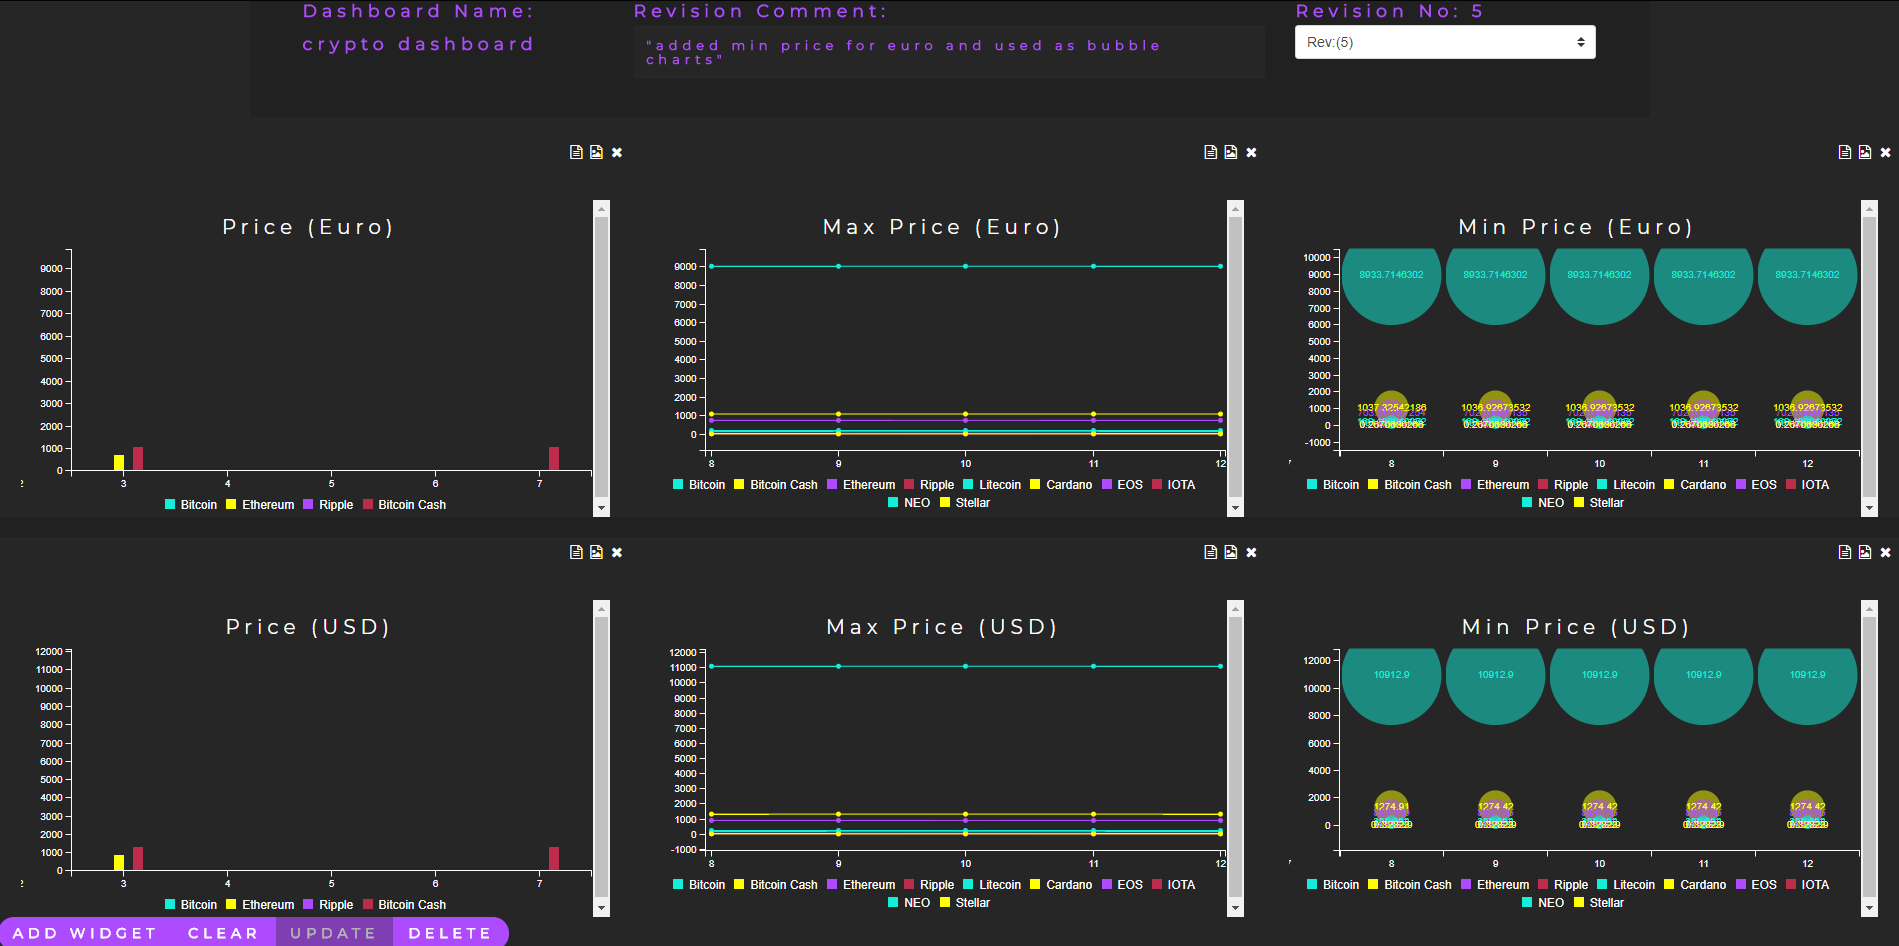
\includegraphics[width=\textwidth,height=\textheight,keepaspectratio]{iris-crypto-agent-dashboard}
\end{center}
A screenshot of the Raspberry Pi agent dashboard in Iris monitoring crypto currencies.
\end{tcolorbox}
\caption{Raspberry Pi agent dashboard in Iris.}
\end{figure}

\subsection{Node.js}
The Node.js agent shows how Iris can integrate with one of the most popular server-side frameworks and how it can monitor the status of the system running Node.js through the npm (node package manager) package `systeminformation'.

\subsubsection{Description}
Due to Node.js' rise in popularity in recent years this agent demonstrates how Iris can easily monitor a system using the `systeminformation' package from npm. The `systeminformation' package offers various levels of detail about the system running Node. Iris' schema for the Node.js agent measures the following attributes:
\begin{itemize}
    \item Operating System Name
    \item Current Uptime of the Operating System
    \item Current CPU Speed
    \item Total Memory Available
    \item Total Memory Free
    \item Total Memory Used
    \item Current CPU Load
\end{itemize}
A full list of all the obtainable attributes through `systeminformation' can be found here \url{https://github.com/sebhildebrandt/systeminformation}.

An important thing to note about this agent is that it takes use of Iris' ability to transform incoming data through scripting. Many of the memory attributes retrieved from `systeminformation' are represented in bytes, this agent uses Iris' centralised transformation abilities to transform the `memFree' attribute to be represented as gigabytes rather than bytes. This script also transforms all the `osName' attributes to be uppercase. Transforming these attributes in Iris through scripting removed the need for a redeployment of the Node.js application.

%Node.js agent transformation script
\begin{figure}[H]
\begin{tcolorbox}
\begin{center}
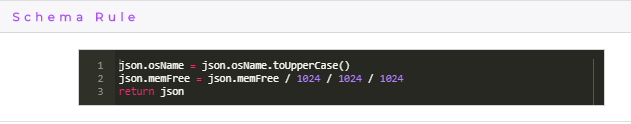
\includegraphics[width=\textwidth,height=\textheight,keepaspectratio]{node-transformation-script}
\end{center}
The transformation script for the Node.js agent which turns the `osName' attribute to uppercase and the `memFree' attribute to be gigabytes rather than bytes.
\end{tcolorbox}
\caption{Node.js agent transformation script.}
\end{figure}

\subsubsection{Linkage with Iris}
The Node.js agent is linked to Iris through a unique REST endpoint specific to the Node.js agent schema. All of the data being sent from the Node.js agent is sent to this endpoint. Once the data enters Iris, Iris will run through it's logic for checking for dashboards and charts associated with the schema and send the data through to the charts. 
%Add a ref to a section where you explain what iris does, so you dont have to keep repeating this for all agents
In this case Iris is monitoring raw data on three charts that are monitoring the current memory free in gigabytes, the current memory used and the current uptime of the system. The other charts display the max memory used over all operating systems and the pie chart shows all the types of operating systems which have run the agent, both of these use Elasticsearch aggregations to calculate the data for the charts.

%Node.js agent schema screenshot in Iris
\begin{figure}[H]
\begin{tcolorbox}
\begin{center}
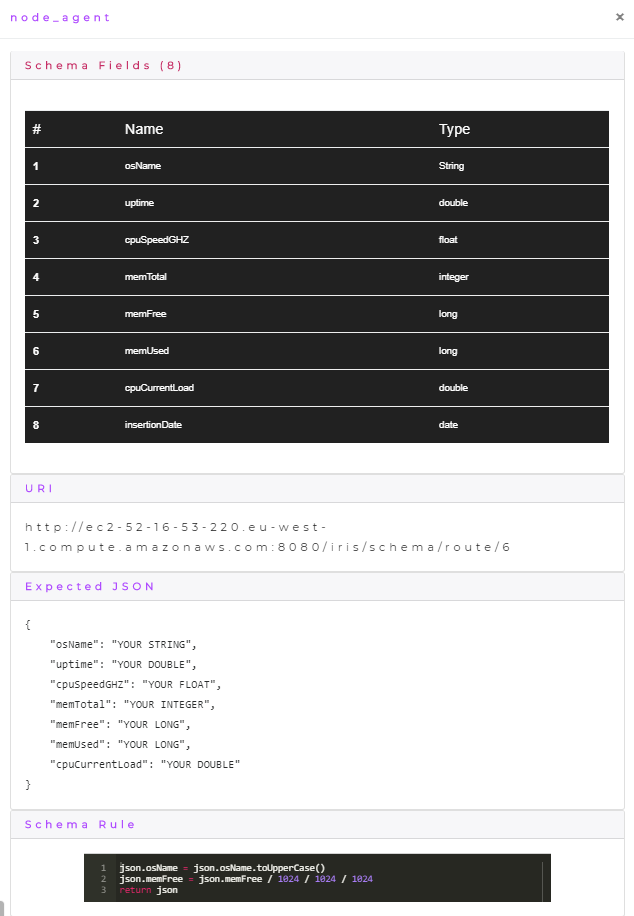
\includegraphics[width=\textwidth,height=\textheight,keepaspectratio]{iris-node-schema}
\end{center}
A screenshot of the Node.js agent schema in Iris.
\end{tcolorbox}
\caption{Node.js agent schema in Iris.}
\end{figure}

%Iris Node agent dashboard screenshot
\begin{figure}[H]
\begin{tcolorbox}
\begin{center}
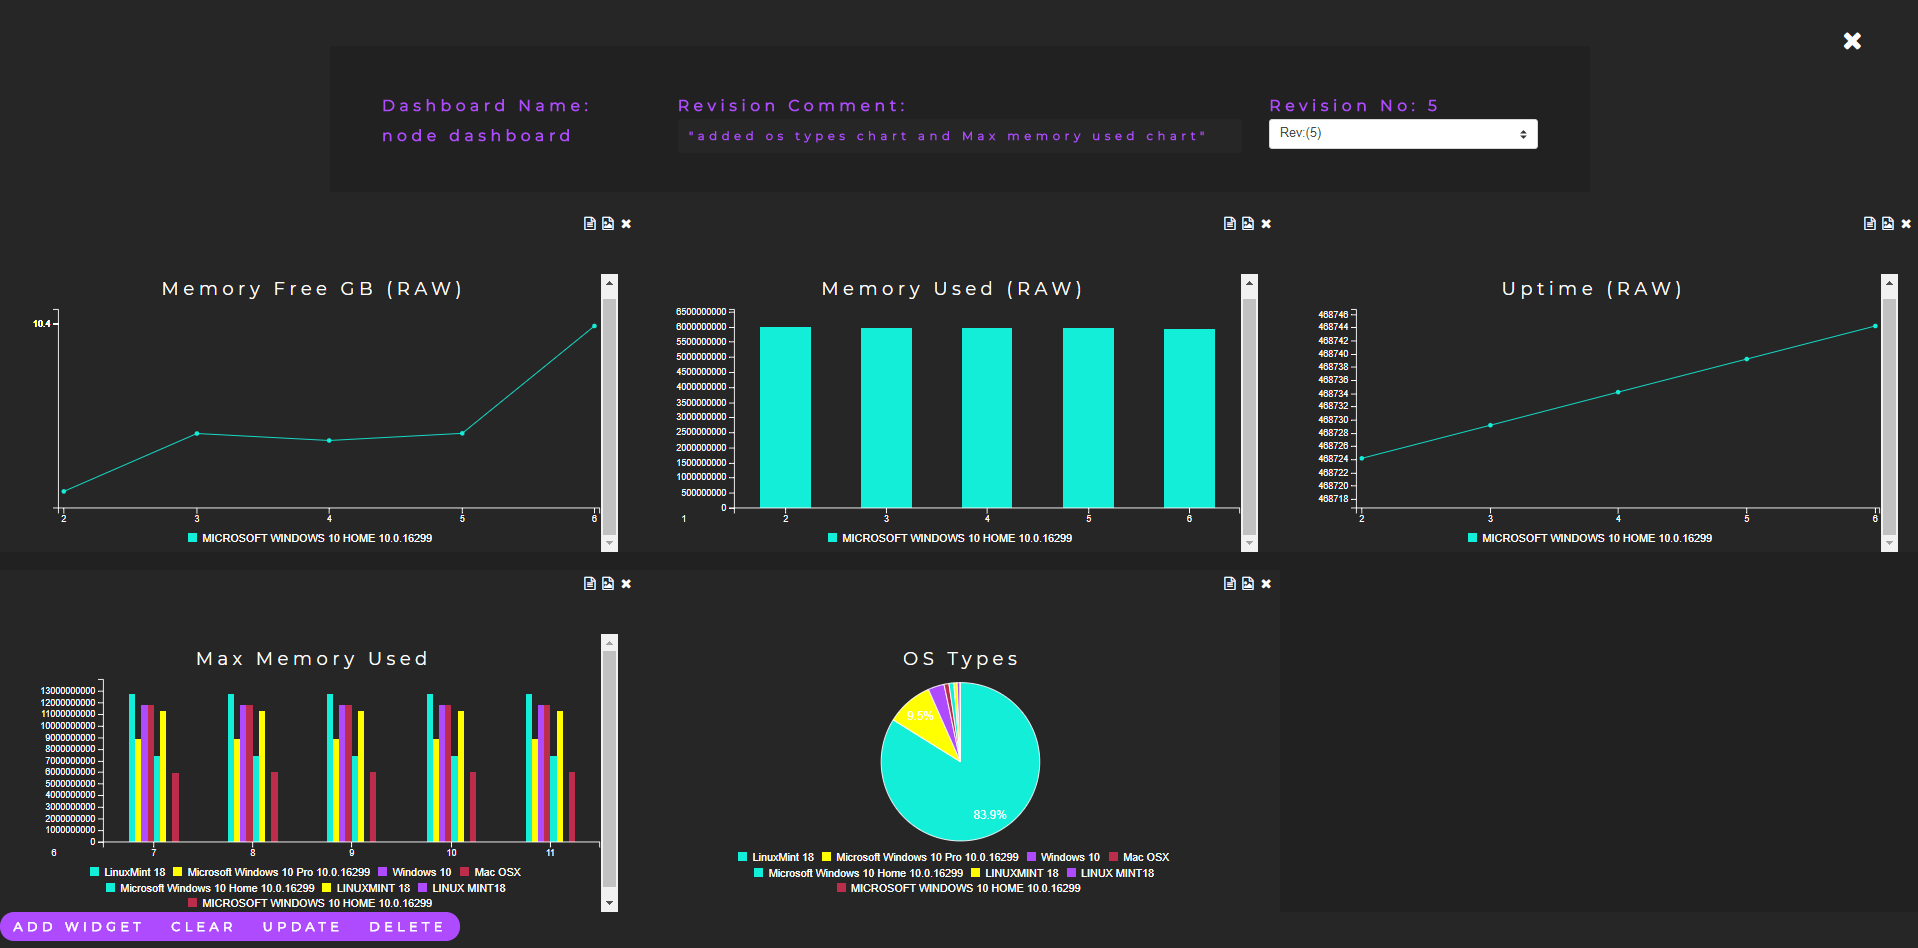
\includegraphics[width=\textwidth,height=\textheight,keepaspectratio]{iris-node-agent-dashboard}
\end{center}
A screenshot of the Node.js agent dashboard in Iris monitoring system information.
\end{tcolorbox}
\caption{Node.js agent dashboard in Iris.}
\end{figure}


\subsection{Selenium}
The Selenium agent demonstrates the versatility of Iris by monitoring the price of a guitar by scraping music store websites and monitoring the price of the guitar. This agent focuses on versatility over complexity.
\subsubsection{Description}
The Selenium agent demonstrates Iris' versatility through the Selenium web driver which is commonly used for web automation and functional testing. In this case Selenium is used in conjunction with a Selenium wrapper called `Selenide' to automate the scraping of music store websites for a specific guitar. On each site the guitar's price is taken from the webpage as well as the name of the music store, the price of the guitar and the name of the music store is then sent to Iris so that it may be monitored.

For more information on Selenide see their site here \url{http://selenide.org/}

\subsubsection{Linkage with Iris}
The Selenium agent is linked to Iris through a unique REST endpoint specific to the Selenium agent schema. All of the data being sent from the Selenium agent is sent to this endpoint. Once the data enters Iris, Iris will run through it's logic for checking for dashboards and charts associated with the schema and send the data through to the charts. 
%Add a ref to a section where you explain what iris does, so you dont have to keep repeating this for all agents
In this case Iris is monitoring raw data on a bar chart. The bar chart monitors the price of the guitar in euro and labels the chart based on the music store website that the price has been scraped from. In this case two sites have been scraped `Thomann' and `MusicStore.de', both sites are competitors and this reflects in the chart as both sites have matched the price of the guitar at the same price.

%Iris selenium agent schema screenshot
\begin{figure}[H]
\begin{tcolorbox}
\begin{center}
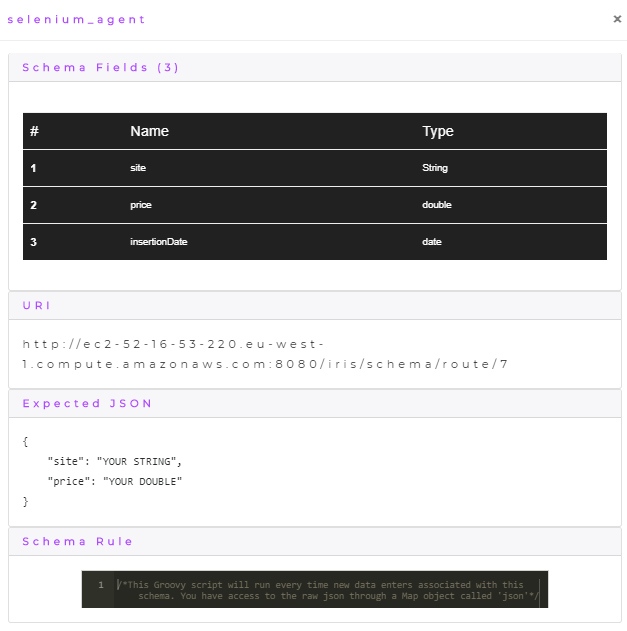
\includegraphics[width=\textwidth,height=\textheight,keepaspectratio]{iris-selenium-schema}
\end{center}
A screenshot of the Selenium agent schema in Iris.
\end{tcolorbox}
\caption{Selenium agent schema in Iris.}
\end{figure}

%Iris selenium agent dashboard screenshot
\begin{figure}[H]
\begin{tcolorbox}
\begin{center}
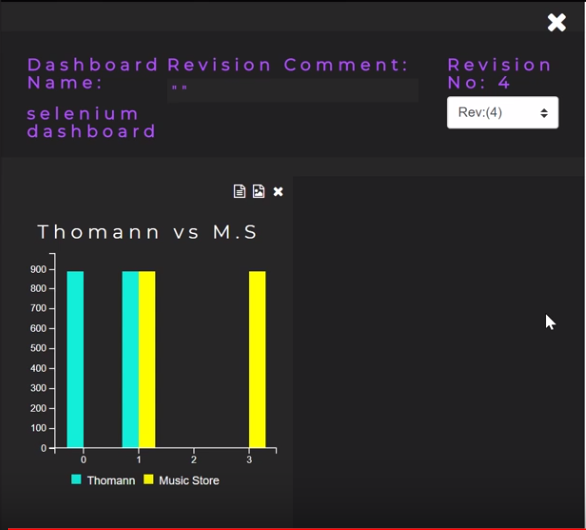
\includegraphics[width=\textwidth,height=\textheight,keepaspectratio]{iris-selenium-dashboard}
\end{center}
A screenshot of the Selenium agent dashboard in Iris.
\end{tcolorbox}
\caption{Selenium agent dashboard in Iris.}
\end{figure}

\subsection{MySQL}
The MySQL agent demonstrates how a user can monitor their database by converting the MySQL `information\_schema' results into JSON and sending them to Iris.
\subsubsection{Description}
The MySQL agent is significant for Iris as this agent was the inspiration for Iris in the beginning, as Onaware developers wanted a way to monitor a remote MySQL database with scripts and be able to monitor the database memory locally with a web application. The MySQL agent is a simple python script that connects to the MySQL instance and monitors all the databases as well as the amount of memory they use. The database name and the amount of memory it currently uses is then sent to Iris to be monitored. The python script is run every day at 8:00pm on the same AWS server that Iris is running on using a cron job.

%MYSQL statement script
\begin{figure}[H]
\begin{tcolorbox}
\begin{minted}{mysql}
SELECT table_schema AS "databaseName", 
ROUND(SUM(data_length + index_length) / 1024 /  1024, 2) as "memoryMB" 
FROM information_schema.TABLES 
GROUP BY table_schema;
\end{minted}
\end{tcolorbox}
\caption{MySQL Agent, MySQL `information\_schema' table query used in iris-mysql.py source code.}
\end{figure}

More information on the MySQL `information\_schema' table can be found here \url{https://dev.mysql.com/doc/refman/5.7/en/information-schema.html}


\subsubsection{Linkage with Iris}
The MySQL agent is linked to Iris through a unique REST endpoint specific to the MySQL agent schema. All of the data being sent from the MySQL agent is sent to this endpoint. Once the data enters Iris, Iris will run through it's logic for checking for dashboards and charts associated with the schema and send the data through to the charts. 
%Add a ref to a section where you explain what iris does, so you dont have to keep repeating this for all agents
The MySQL agent dashboard monitors the average memory taken up by each database in the MySQL instance and displays the results as a line chart in Iris.
%Iris mysql schema screenshot
\begin{figure}[H]
\begin{tcolorbox}
\begin{center}
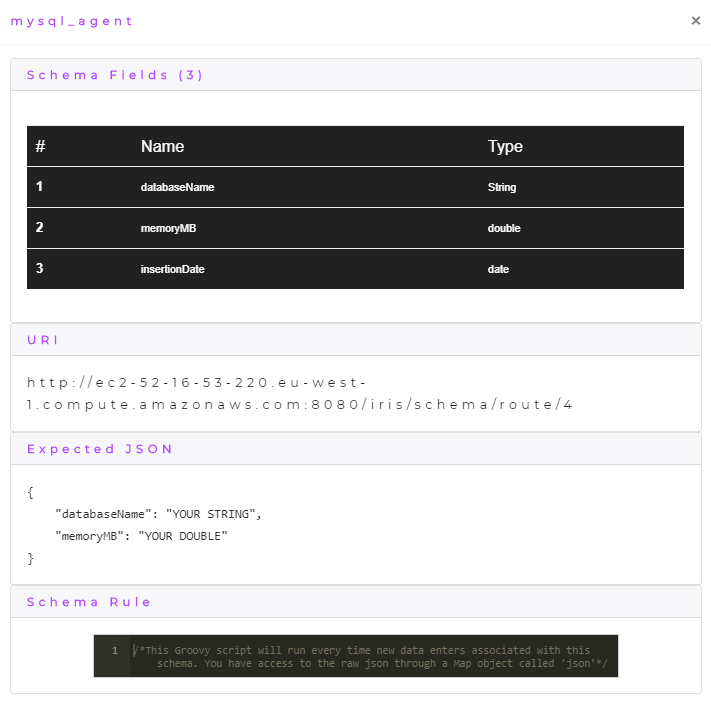
\includegraphics[width=\textwidth,height=\textheight,keepaspectratio]{iris-mysql-schema}
\end{center}
A screenshot of the MySQL agent schema in Iris.
\end{tcolorbox}
\caption{MySQL agent schema in Iris.}
\end{figure}

%Iris mysql dashboard screenshot
\begin{figure}[H]
\begin{tcolorbox}
\begin{center}
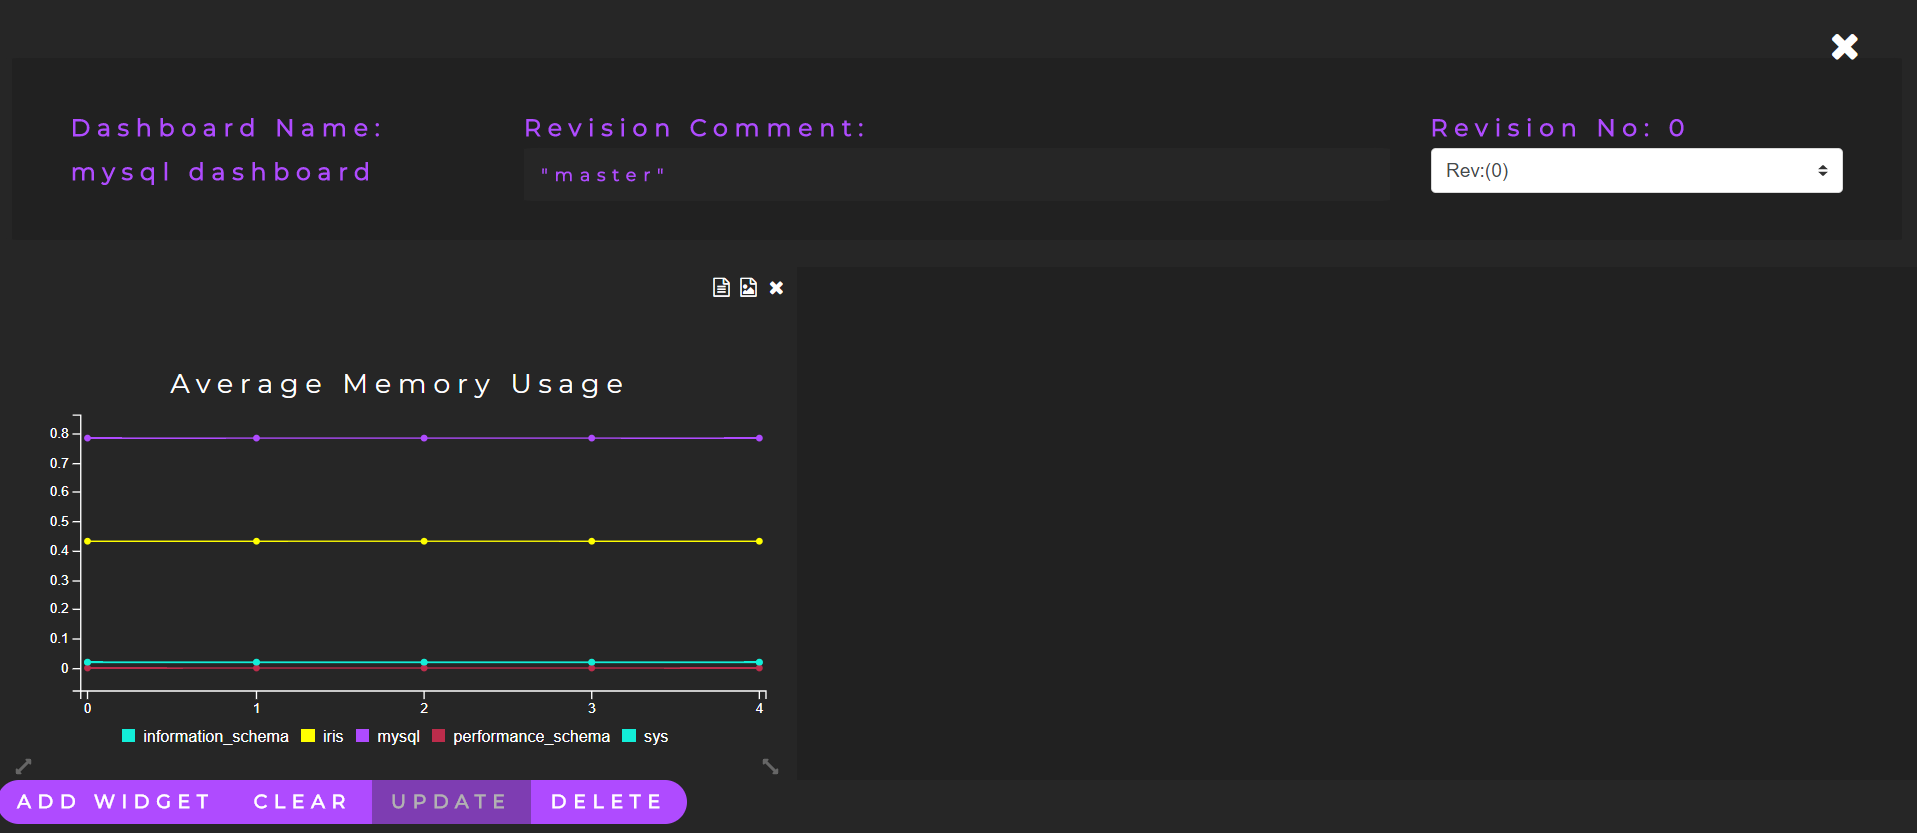
\includegraphics[width=\textwidth,height=\textheight,keepaspectratio]{iris-mysql-dashboard}
\end{center}
A screenshot of the MySQL agent dashboard in Iris.
\end{tcolorbox}
\caption{MySQL agent dashboard in Iris.}
\end{figure}

\chapter{Conclusions}


%No cite prints all references even if they are not in the document!!
\nocite{*}
\printbibliography

%%%%%%%%%%%%%%%%%%%%%%%%%%%%%%%%
\clearpage

\begin{appendices}

\end{appendices}
\end{document}
